\section{Automatic Testing}

\subsection{Übersicht über die Tests}

\begin{description}
	\item[typed] Deklaration von Paketen zur Weiterverbreitung
	\item[myPy] Checking for Typins
	\item[flake8] Testen auf Code Style
	\item[Pytest] Eigene Unit Tests
	\item[Tox] Tests in unterschiedlich konfigurierten Python Umgebungen
	\item[GitHub Action] Automatische Durchführung der Tests
\end{description}
	
\subsubsection{Nicht behandelte Themen}
In der ersten Version dieses Kapitels werden die Themen: \textit{Hocks, welche automatische Dokumentation, Build, Skripte etc. durchführen} und \textit{Deployment Prozess} nicht behandelt.

\subsubsection{Mehrwert von Tests}
Mit der Anwendung des Konzepts \textit{Automatic Testing} soll möglich sein, dass Programme automatisch getestet werden bei einem Merge oder Commit Vorgang. Die Entwickler herhalten einen ersten Einblick, ob das Programm den eigen gesetzten Anforderungen genügen.\footnote{
 Github bietet die Möglichkeit, dies direkte visuell einzusehen, ob der Test erfolgreich war.
\begin{figure}[H]
	\centering
	
\includegraphics[scale = 0.6]{attachment/chapter_2/Scc073}
	\caption{Bsp.: Zielsetzung: Ergebnis der Test anzeigen}
\end{figure}
}

\subsubsection{Übersicht über Konfigurationen}
Für den Test werden mehre Konfigurationen hinzu, welche den Testdurchlauf regeln. Dies ist nicht einheitlich gehandhabt bei Paketen. Manche benötigten ihre Konfiguration in der \textit{setup.cfg} Datei andere in der \textit{pyproject.toml} Datei und andere benötigen gleich eigenen Konfigurationsdateien. Nach Ansicht von mCoding ist, dass die meisten Konfigurationen in der \textit{pyprojekt.toml} Datei hinterlegt werden müssen. In der \textit{setup.cfg} Datei werden die Meta Daten hinterlegt.

\begin{figure}[H]
	\centering
	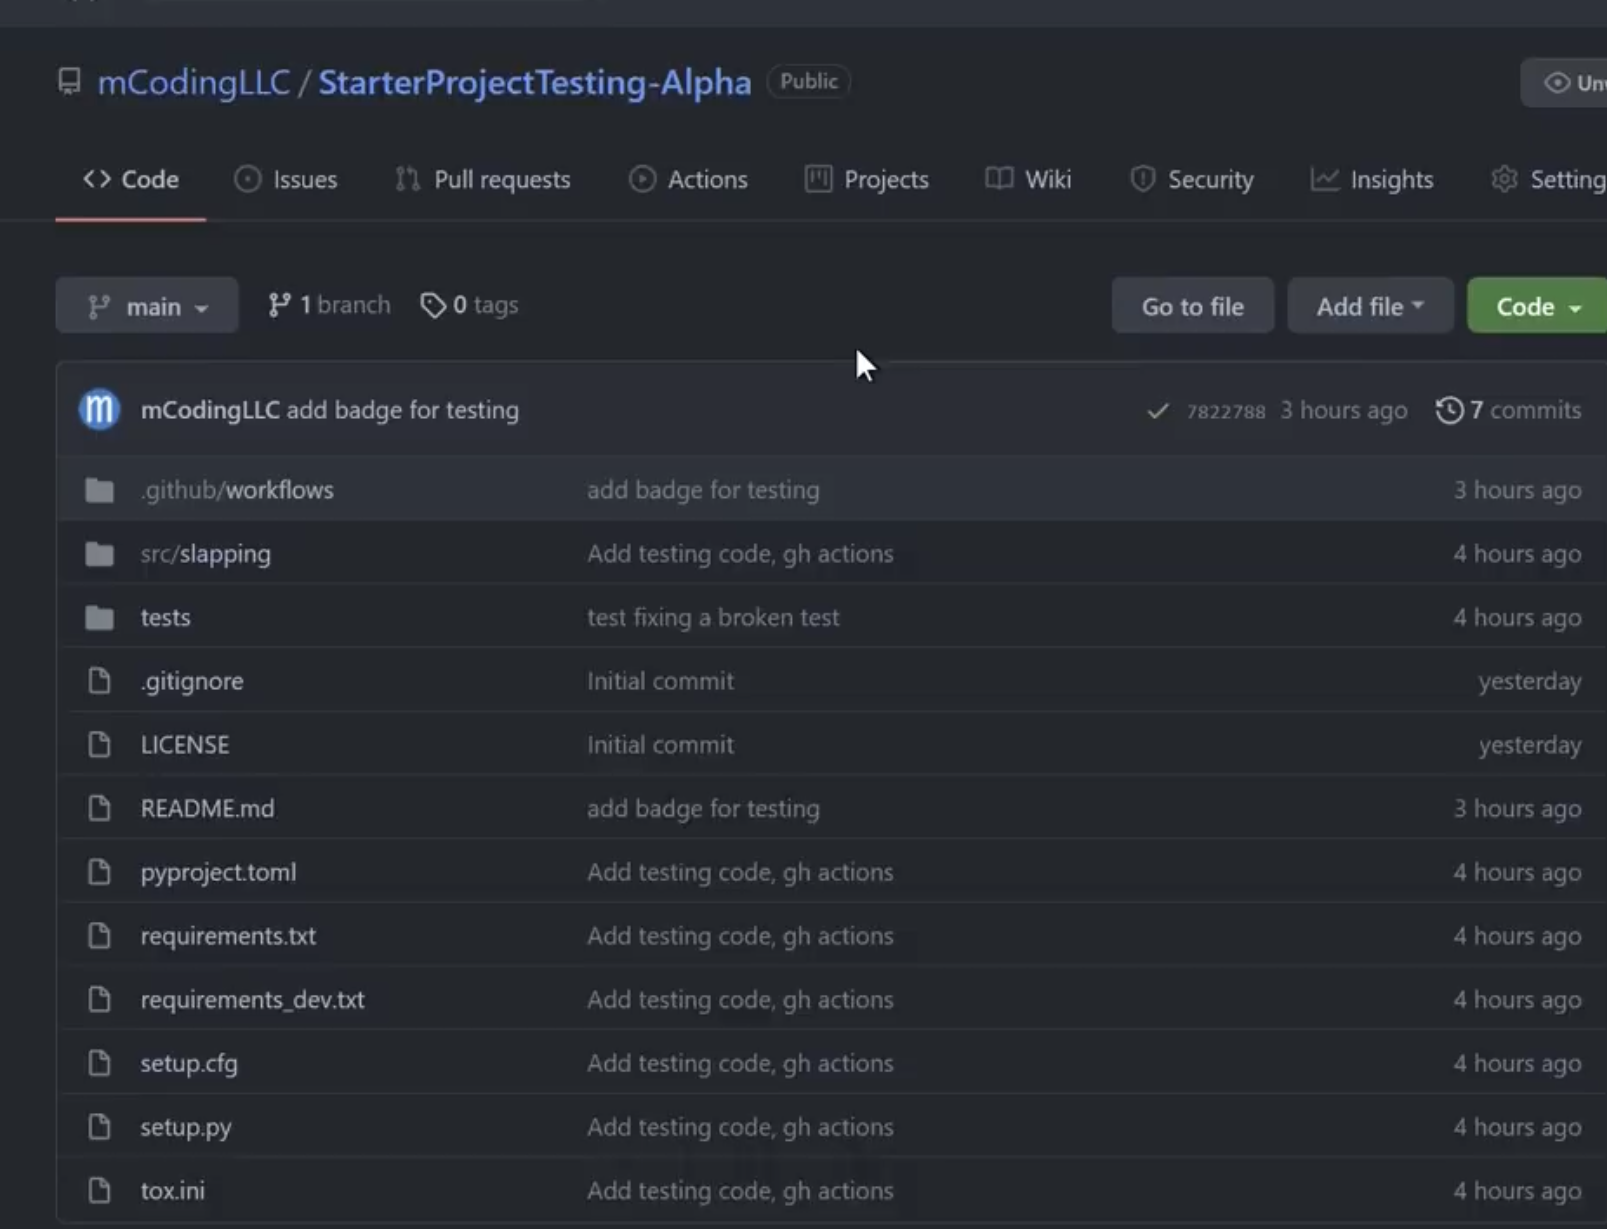
\includegraphics[scale = 0.2]{attachment/chapter_2/Scc066}
	\caption{Bsp: Für Repository Konfiguriert für Tests}
\end{figure}

\subsubsection{Dev Requirements} Für den Test werden die Bibliotheken für die Tests benötigt. Dieser werden jedoch nicht im laufenden Betrieb benötigt. Daher wird mit \textit{requirements}$\_$\textit{dev.txt} und \textit{conda}$\_$\textit{requirements}$\_$\textit{dev.yml} eine separate Anforderungen an die benötigten Bibliothken gestellt.

\begin{lstlisting}[style=Config, caption={Bsp. requirements\_dev.txt; Paket Requirments für Tests}, captionpos=b]
...
mypy==0.910
flake8==3.9.2
tox==3.24.2
pytest==6.2.5
pytest-cov==2.12.1
...
\end{lstlisting}

Weil es sich hier um neue Packet handelt, werden die Abhängigkeiten unter \textit{setup.cfg} hinterlegt.
\begin{lstlisting}[style=Config, caption={Bsp. Separate Abhängigkeiten für Tests}, captionpos=b]
...
[options.extras_require]
testing = 
	mypy>0.910
	flake8>3.9
	tox>3.24
	pytest>=6.0
	pytest-cov>=2.0
\end{lstlisting}

\subsection{Small Test Libaries}
\subsubsection{typed}
Um Pakete für die Verteilung aufzubereiten wird unter \textit{setup.cfg} angegeben, dass das Modul dem Standard nach \textit{PEP 561} folgt:
\begin{lstlisting}[style=Config]
...
[options.package_data]
slapping = py.tyed
...
\end{lstlisting}
Im Verzeichnis wird die Datei \textit{py.typed} hinterlegt.
\begin{figure}[H]
	\centering
	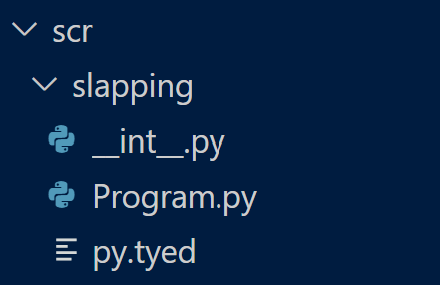
\includegraphics[scale = 0.6]{attachment/chapter_2/Scc075}
\end{figure}
Diese ist eine Referenzdatei. Für mehr Informationen siehe \textbf{PEP 561}.

\subsubsection{mypy}
\paragraph{Konfiguration - toml} Für \textit{mypy} gilt das gleich wie für \textit{pytest}, die Konfiguration wird die \textit{toml} Konfiguration geschrieben:
\begin{lstlisting}[style=Config]
...

[tool.mypy]
mypy_path = "src"
check_untyped_defs = true
disallow_any_generics = true
ignore_missing_imports = true
no_implicit_optional = true
show_error_codes = true
strict_equality = true
warn_redundant_casts = true
warn_return_any = true
warn_unreachable = true
warn-unused_configs = true
no_implicit_reexport = true
\end{lstlisting}

Wenn die Tests konfiguriert sind und die \gls{VEN} für die Testmodule angelegt ist, können die Test über das Terminal durchgeführt werden.

\paragraph{Erklärung mypy} ist ein Modul, welches \textbf{Type Hints} überprüft.
Python ist eine dynamische Programmiersprache. Dies bedeutet, dass Angaben über den Typ von Variablen nicht explizit getätigt werden müssen. Anders ist dies bei Programmiersprachen wir \textit{C++}. Mit \textit{mypy} kann eine Überprüfung von \textbf{statischen Type hints} überprüft werden. Dies kann je nach Einstellungen und Optionen in genauer Granularität vorgenommen werden.\footnote{
Mypy is an optional static type checker for Python that aims to combine the benefits of dynamic (or "duck") typing and static typing. Mypy combines the expressive power and convenience of Python with a powerful type system and compile-time type checking. Mypy type checks standard Python programs; run them using any Python VM with basically no runtime overhead.
} 
Es kann auf einzelne Skript

\begin{lstlisting}[style=CMD]
mypy <skript name>.py
\end{lstlisting}

oder ganze Verzeichnisse
\begin{lstlisting}[style=CMD]
	mypy scr
\end{lstlisting}
angewandt werden. Für die Konfiguration wird die \path{myproject.toml} konfiguriert.

Die Grundeinstellung von mypy ist, dass dynamische ausgewiesene Funktionen nicht als Fehler ausgegeben werde.

\begin{lstlisting}[style=python, caption={Example dynamical typed function}, captionpos=b]
def addition (a, b):
	return a + b
\end{lstlisting} 

\paragraph{Am Beispiel} einer einfachen Funktion, welche zwei Zahlen addiert, kann mypy angewandt werden.
\begin{figure}[H]
	\centering
	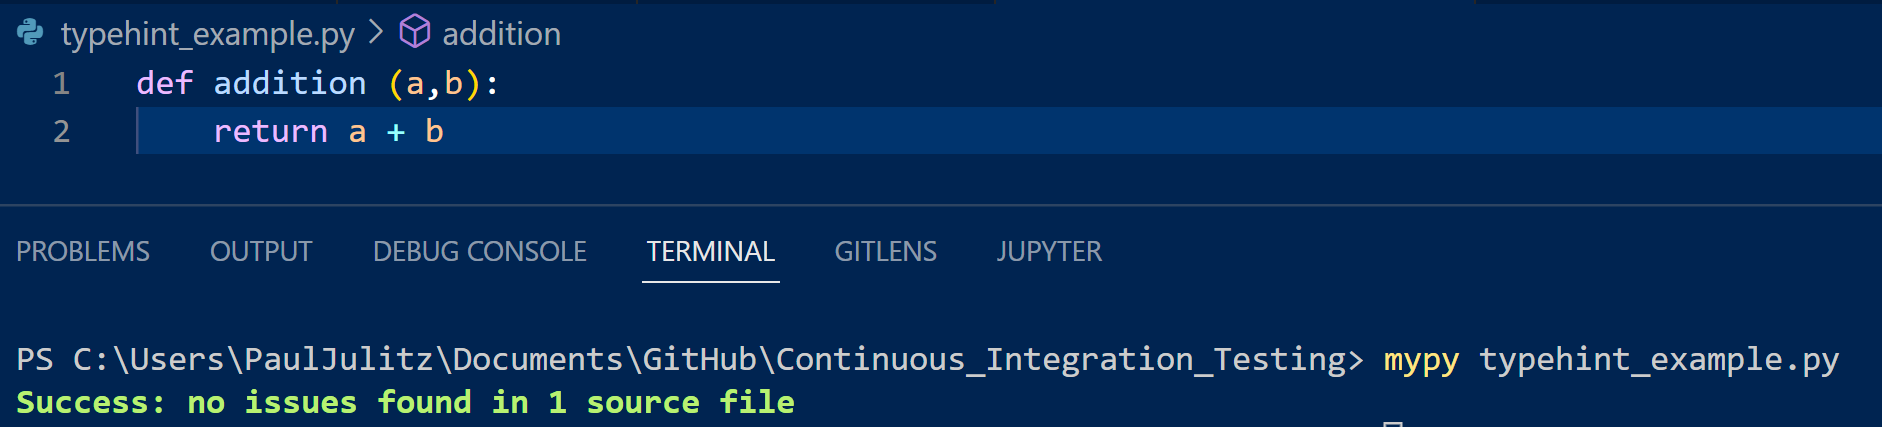
\includegraphics[scale = 0.6]{attachment/chapter_2/Scc078}
	\caption{Type hint check - Variante 1}
\end{figure}
In der Variante 1 werden keine Type Hints gesetzt und die Type Adressierung funktioniert dynamisch.

Werden die Type Hintes $a:int$ und $b:dict$ gesetzt, würde in Python selbst kein Fehler angezeigt, bis es zur Ausführung des Programms. Mit \textit{mypy} kann dies erkannt werden.
\begin{figure}[H]
	\centering
	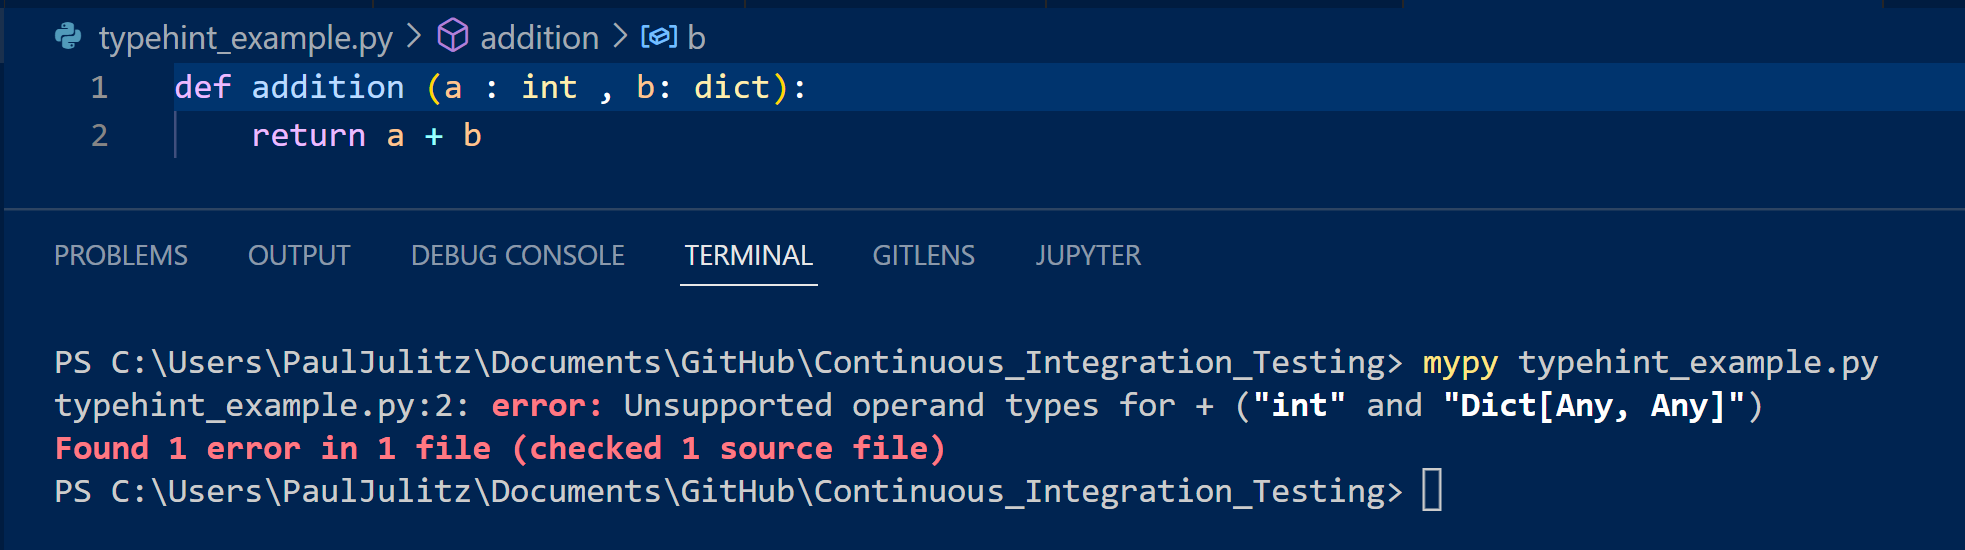
\includegraphics[scale = 0.6]{attachment/chapter_2/Scc079}
	\caption{Type hint check - Variante 2}
\end{figure}
Im Ideal Fall sind die beide Type Hints richtig hinterlegt.
\begin{figure}[H]
	\centering
	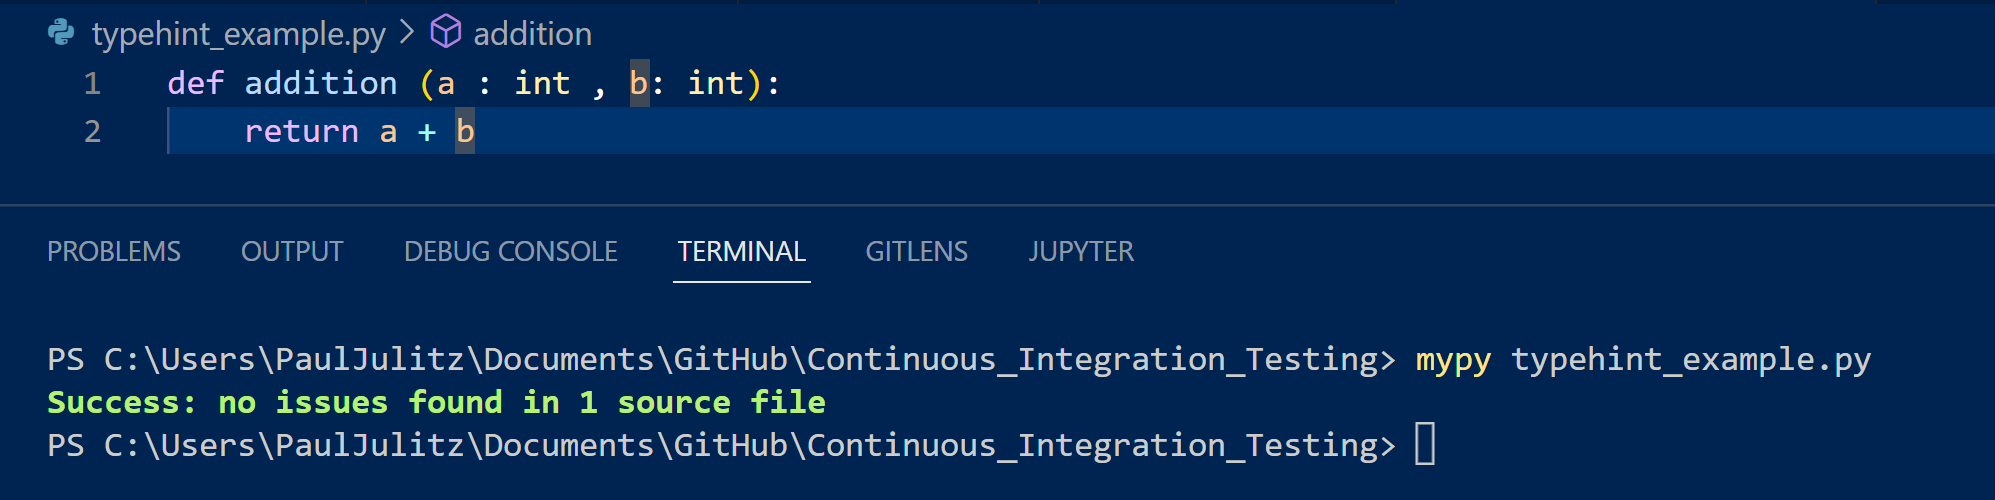
\includegraphics[scale = 0.6]{attachment/chapter_2/Scc080}
	\caption{Type hint check - Variante 3}
\end{figure}

Wir eine Option für zwei mögliche Type Hints
\begin{lstlisting}[style=python]
def addition (a : int | None , b: int) -> int:
	# Union symbole requires Python Version 3.10 or higher. 
	return a + b
\end{lstlisting}
wird ebenso eine Fehlermeldung angezeigt. Dies kann umgangen werden, in dem für beide Fälle berücksichtigt werden.
\begin{lstlisting}[style=python]
def addition (a : int | None , b: int) -> int:
	# Union symbole requires Python Version 3.10 or higher. 
	if not a
		return 0 
	return a + b
\end{lstlisting} 

Für das den hier beschriebenen Anwendungsfall wird 
\begin{lstlisting}[style=CMD]
mypy scr
\end{lstlisting}
ausgeführt. Für die Skripte \textit{$\_\_$init$\_\_$.py} und \textit{Programm.py} wird der Test durchgeführt. Das Ergebnis ist \textcolor{vbagreen}{Success}.\\


\subsubsection{flake8}
\paragraph{Konfiguration - setup}
Diese wird in \textit{setup.cfg} hinterlegt. Eine Basiskonfiguration ist
\begin{lstlisting}[style=Config]
...
[flake8]
max-line-length=160
exclude = .git
extend-ignore = W292, E266
...
\end{lstlisting} 

Mit \textit{max-line-length} setze die Zeilenlänge fest, wie lange eine Eintrag sein kann. Mit der \textit{exclude} Option werden Daten und Verzeichnise festgelegt, welche nicht überprüft wurden.

\paragraph{Erläuterung}
Mit \textit{flake8} wird der Style eines Python Skripte überprüft.\\

\textbf{Hinweis:} Der Style eines Python Skript ist mit der Version von Python verbunden. Mit einer geänderte Version von Python wird auch die entsprechende Version von \textit{flake8} benötigt.\\

Mit \textit{flake8} werden
\begin{description}
	\item[Coding Standards (PEP8)]
	\item[Programming $"$errors$"$ und] Unter einem Programmierungsfehler wird hier eine ungenutzte Bibliothek oder ungenutzte Variablen verstanden.
	\item[textit{cycolmatic complexity} kontrolliert] Dies ist eine Metrik, welche die Anzahl der unabhängigen Pfade in einem Programm misst. Ein niedriger Nummer bedeutet, dass das Programm leichter zu verstehen ist und weniger Aufwand bedeutet, bei einer Modifikation.
\end{description}

Unter \href{https://simpleisbetterthancomplex.com/packages/2016/08/05/flake8.html}{How to use flake} sind weitere Ausführungen zu finden.\\

Mit $\#$ \textit{noqa} oder mit einem spezifischen Fehlercode z.B. $\#$ \textit{noqa: F401} wird ein Code-Zeile im Skript ignoriert.

\begin{lstlisting}[style=python]

class ProfilesConfig(AppConfig):
    name = 'cmdbox.profiles'
    verbose_name = _('profiles')

    def ready(self):
        import cmdbox.profiles.signals.handlers  # noqa: F401
\end{lstlisting}

\paragraph{Anwendung}
Mit dem Befehl 
\begin{lstlisting}[style=CMD]
flake8
\end{lstlisting}

wird \textit{flake8} auf das komplette Projekt angewandt. Mit dem Verweis auf ein Verzeichnis kann die Kontrolle eingegrenzt werden. 

\begin{lstlisting}[style=CMD]
flake8 scr/
\end{lstlisting}

Der Output wird in der Form

\begin{lstlisting}[language={}]
.\typehint_example.py:1:15: E203 whitespace before ':'
.\typehint_example.py:1:21: E203 whitespace before ','
.\typehint_example.py:2:60: W291 trailing whitespace
.\typehint_example.py:5:1: E305 expected 2 blank lines after class or function definition, found 1
.\typehint_example.py:5:15: W292 no newline at end of file
.\build\lib\slapping\Program.py:40:13: W292 no newline at end of file
.\scr\slapping\Program.py:40:13: W292 no newline at end of file
.\tests\test.py:1:21: W292 no newline at end of file
.\tests\test_slapping.py:4:1: E302 expected 2 blank lines, found 1
.\tests\test_slapping.py:5:6: E111 indentation is not a multiple of 4
.\tests\test_slapping.py:5:6: E117 over-indented
.\tests\test_slapping.py:6:6: E111 indentation is not a multiple of 4
.\tests\test_slapping.py:7:6: E111 indentation is not a multiple of 4
.\tests\test_slapping.py:8:6: E111 indentation is not a multiple of 4
.\tests\test_slapping.py:9:6: E111 indentation is not a multiple of 4
.\tests\test_slapping.py:10:6: E111 indentation is not a multiple of 4
.\tests\test_slapping.py:11:6: E111 indentation is not a multiple of 4
.\tests\test_slapping.py:11:64: W292 no newline at end of file
\end{lstlisting}

angezeigt. Die Formatierung folgt der Logik

\begin{center}
	\textit{file path} : \textit{linie number} : \textit{column number} : \textit{error code} : \textit{short description}
\end{center}

Fehlercode Prefix:
\begin{description}
	\item[E<...>] Pep8 errors
	\item[W<...>] Pep8 warning
	\item[F<...>] PyFlake8 Code
	\item[C9<...>] McCabe complexity plugin 
	\item[N8<...>] Naming convention plugin (pep8)
\end{description}

\paragraph{Beispiel: E111 indentation is not a multiple of 4}
Ein Einrückung in einem Python Skript wird mit vier Leerzeichen als Standard gesetzt. Über die \gls{IDE} Visual Studio kann die $"$Indentation setting$"$ mit einem Tab erfolgen. In diesem Programm

\begin{figure}[H]
	\centering
	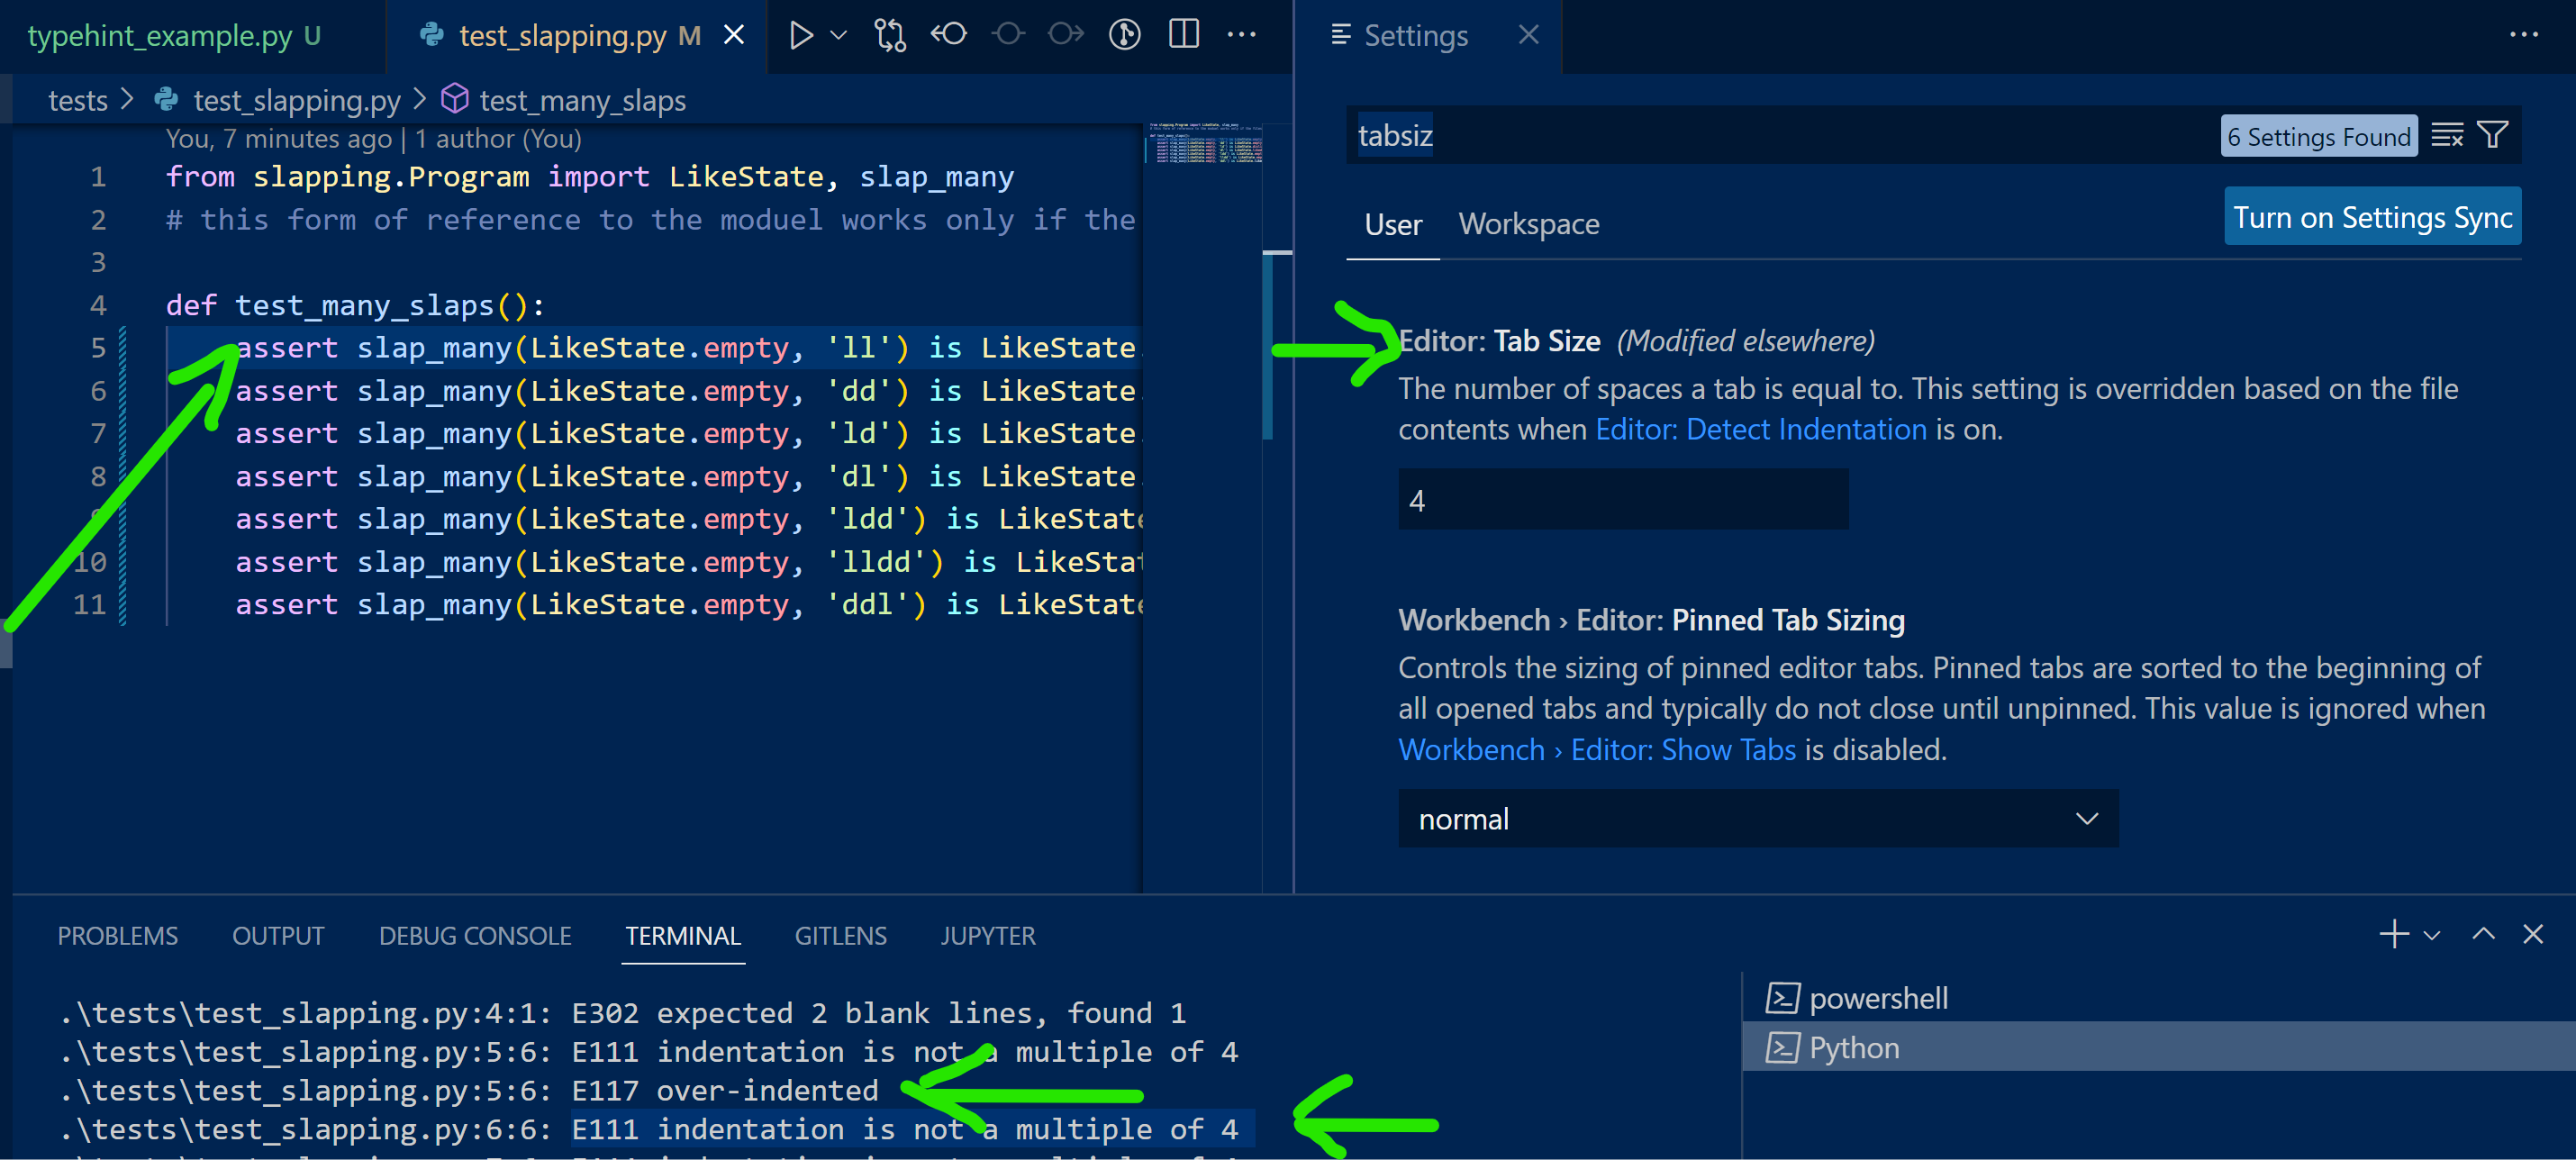
\includegraphics[scale = 0.6]{attachment/chapter_2/Scc081}
	\caption{Behebung E111}
\end{figure}

\paragraph{Beispiel: W292 no newline at end of file}
In PEP8 wird angegeben, dass am Ende einer Skript Datei eine leere Zeile kommt.

\begin{lstlisting}[style=python , caption={Schlechtes Beispiel}, captionpos=b]
class ProfilesConfig(AppConfig):
    name = 'cmdbox.profiles'
    verbose_name = _('profiles')

    def ready(self):
        import cmdbox.profiles.signals.handlers  # noqa: F401
\end{lstlisting}

\begin{lstlisting}[style=python, caption={Gutes Beispiel}, captionpos=b]
class ProfilesConfig(AppConfig):
    name = 'cmdbox.profiles'
    verbose_name = _('profiles')

    def ready(self):
        import cmdbox.profiles.signals.handlers  # noqa: F401
        
\end{lstlisting}
Der Standard W292 verlangt hingegen kein leere Zeile am Ende.

\section{tox-conda}

\subsection{Motivation}
Mit \textit{tox} soll die Testungen Python automatisiert werden. Als Frontend soll tox dienen mit CI-Server zu kommunizieren, um Testungen automatisch ohne ohne großes zutun zu verwalten. Es werden verschiedene Virtuelle Umgebungen erstellt, welche unter verschiedenen Konfigurationen die Testungen des Codes vornehmen.\\

Das Plug-in \textit{tox-conda} wird verwendet, wenn die Verwaltung von der \gls{VEN} durch conda betrieben wird.


\subsection{Allgemeine Konfiguration Begrifflichkeiten (Short)} 
Für \textit{tox}/ \textit{tox-conda} wird die Konfiguration \textit{tox.ini} erstellt. Mit \textit{tox-conda} werden mehrer $"$settings$"$ unter \textit{testevn} zur Verfügung gestellt. Für die weitere Erklärung wird nur
\begin{description}
	\item[cond$\_$env], gibt an, wo und welche \textit{conda-evn.yml} Datei für die Erstellung der \gls{VEN} in conda genutzt wird.
	\item[$\left\lbrace \right. $toxinidir$\left.\right\rbrace$] Gibt den Pfad zurück, in welchem tox ausgeführt wurde. Wenn Tox im Hauptverzeichnis der Applikation liegt, dann wird dieser Pfad zurückgegeben.
\end{description}
relevant sein. Weitere Einstellungen, wie conda$\_$deps, conda$\_$channel, können unter \href{https://github.com/tox-dev/tox-conda} zur Verfügung gestellt werden.

\subsection{Bsp.: Grundfunktionalität}
Diese Beispiel dient die Grundfunktionalität von tox gezeigt. Diese zeigt die Automatisierung der Installation einer \gls{VEN} und die Ausführung eines Kommands.\\

In der tox Konfigurationsdatei, \textit{tox.ini}, wird festgelegt, dass die \gls{VEN} für die Python Version 3.7 aufgesetzt werden soll. Die Abhängigkeiten (deps) werden über die requirements$\_$dev.txt Datei installiert. Dies sind alle Packet, welche benötigt werden, um den Test durchzuführen. Wenn die Erstellung der \gls{VEN} fertig ist und alle benötigten Packete installiert werden, wird der Befehl \textit{pytest} ausgeführt. Diese drei Schritte
\begin{itemize}
	\item Erstellen einer \gls{VEN},
	\item Installation aller Abhängigkeiten und 
	\item die Ausführung von Kommandozeilen Befehle
\end{itemize}
werden in der \textit{tox.ini} festgehalten.

\begin{lstlisting}[style=Config]
# ============================================================================
# TOX CONFIGURATION: behave
# ============================================================================
# REQUIRES: pip install tox

[tox]
envlist = py37
# Environment name python3.7

[testenv] 									# Standard python enviroments
deps=	-rrequirements_dev.txt 				# delivers the dependencies
commands = pytest							# Runs command
\end{lstlisting}


Vollständigkeitshalber, die folgende Applikationsstruktur sieht wie folgt aus.
\begin{figure}[h]
	\centering
	\resizebox{0.2\textwidth}{!}{% Faktor zum Skalieren
		\begin{forest}
			for tree={
				font=\sffamily,
				grow'=0,
				folder indent=0.9em,
				folder icons,
				edge=densely dotted
			}
			[Application
			[test
				[$\_\_$init$\_\_$.py, is file]
				[test$\_$roman.py, is file]
			]
			[scr/
				[$\_\_$init$\_\_$.py, is file]
				[roman.py, is file]
			]
			[requirements.txt, is file]
			[requirements$\_$dev.txt, is file]
			[Readme.md, is file]
			]
		\end{forest}
	}%
	\caption{Bsp.: Rudimentärer Aufbau einer Applikation.}
\end{figure}

\subsection{Bsp.: Erweitere Befehle}

\begin{itemize}
	\item Der Eintrag \textit{postargs} erlaubt über das Kommando, welches tox ausführt, Argumente einzufügen. Es kann ein spezifischer Schlüsselbegriff verwendet werden. Dieser wird über \textit{--} aktiviert.
	\item Die pytest Option --basetemp weißt pytest an, das Verzeichnis zu überschreiben, bei jedem Durchlauf von pytest.
	\item Die Option toxinidir verweißt auf das Verzeichnis, in welchem tox.ini liegt. Bei den Installationsbefehlen wird es als Standard angenommen. Es ist daher im unteren Beispiel redundant.\footnote{
	\href{https://tox.wiki/en/latest/example/basic.htmldepending-on-requirements-txt-or-defining-constraints}{Quelle}
}
	%TODO Test
	% Funktioniert die CI-Pipeline auch ohne den Vermerk mit toxinidir?
	\item Installation der requirements Datei. Dies muss ohne Leerzeichen zu r gesetzt werden, sonst würde tox dies als zwei deps sehen.
	\item \textit{setenv} deklariert für jede Zeile eine Variablen.\footnote{
		Es ist unklar, warum es für den pythonpath genutzt wird.
	}
\end{itemize}


\begin{lstlisting}[style=Config]
# ============================================================================
# TOX CONFIGURATION: behave
# ============================================================================
# REQUIRES: pip install tox

[tox]
envlist = py37
# Environment name python3.7

[testenv] 									# Standard python enviroments
deps=	-r{toxinidir}/requirements_dev.txt # delivers the dependencies
commands = pytest --basetemp={envtmpdir} {postargs:varialbe} # clear temp directory
setenv = 
	PYTHONPATH = {toxinidir}				# currently unclear, why it is used
\end{lstlisting}

Im einfachsten Fall wird nur tox ausgeführt ohne Extras.
\begin{lstlisting}[style=CMD, caption={Bsp.: Befehl zum Ausführen von tox}, captionpos=b]
tox 
\end{lstlisting}

Unter Einsatz des positionalen Eintrages, wird diese übergeben.
\begin{lstlisting}[style=CMD, caption={Nur fstrings tests werden ausgeführt}, captionpos=b]
tox -- variable -k fstring
\end{lstlisting}
Es muss kein Substitutionsname angegeben werden. Alles was nach -- kommt, wird eingesetzt. \footnote{
	Weiter Beispiele könnten unter tox gefunden werden. \href{https://tox.wiki/en/latest/example/pytest.html}{Quelle}
}

\subsection{Bsp.: Grundfunktionalität mit conda}
Das simple Beispiel wir das Add-In \textit{tox-conda} verwendet. Diese nutzt conda für den Installationsprozess. Dafür wird die \gls{.yaml} verwendet. \footnote{
	Hierzu kann unter \href{https://github.com/tox-dev/tox-conda/pull/48 mehr nachgelesen werden.}; 
}
\footnote{
	Bei der lokalen Ausführung (Vermutung) muss eine erst Umgebung angelegt werden, welche tox und tox-conda zu mindestens enthält.
}

\begin{lstlisting}[style=Config]
[tox]
envlist = py37						# Single environment

[testenv]								# default comand for python versions
conda_env = requirements_dev.yml	# installs dependencies
commands = pytest 
\end{lstlisting}
%TODO Test
% Ob es so über conda funktioniert, ist unklar. -r wird nicht angewandt


\subsection{Bsp. Vorherige Ausführung}
Für die Entwicklung-\gls{VEN} wird \textit{tox-conda} über pip 
\begin{lstlisting}[style=CMD]
pip install tox-conda
\end{lstlisting}
oder conda 
\begin{lstlisting}[style=CMD]
conda install -c conda-forge tox-conda
\end{lstlisting}
oder über conda$\_$requirments$\_$dev.yml
\begin{lstlisting}[style=Config, caption={Conda-Requirment-Dev für tox-conda}, captionpos=b]
	name: Continuous_Integration
	dependencies:
	- requests=2.26.0
	- pip=22.1.2
	- python=3.8.13
	- tox-conda=0.9.2
	- pip:
	- pip install -r requirments_dev.txt
\end{lstlisting}
%TODO Test
%pip install -r requirments.txt herausnehmen, wenn pip install -e . ausgeführt wird und die Setup.py startet, wird pip install -r requirments.txt ebenso installiert. Wie sich dies in Kombination mit den anderen Konfiguration auswirkt ist unklar. Wie kann jetzt die Conda umgebung erstellt werden.

\subsection{Bsp.: Multiple Umgebungen}
Im Folgenden wird für jedes Testmodul eine eigene \gls{VEN} erstellt.
Die sind eigenen Umgegeben, welche mit jeweiligen Kommands verbunden sind. 

\begin{lstlisting}[style=Config, caption={Own Env}, captionpos=b]
...
[tox]
envlist = py37, py38, flake8, mypy	# Plus own Envi
...

[testenv:flake8]
basepython = python3.6
deps = flake8
commands = flake 8 scr tests

[testenv:mypy]
basepython = python3.6
deps=	-r{toxinidir}/requirements_dev.txt # delivers the dependencies
commands = mypy scr
\end{lstlisting}

\section{pytest}
\subsection{Allgemein}
\paragraph{Setup pyprojekt.toml} \label{par:Setup pyprojekt.toml} 
Es gibt mehrere Möglichkeiten die Konfiguration von \textit{pytest} zu hinterlegen. 

\begin{lstlisting}[style=Config, caption={Beispiel pyproject.toml; Slapping pytest config}, captionpos=b]
...
[tool.pytest.ini_options]
addopts = "--cov=slapping"
testpaths = [
	"tests",
]
\end{lstlisting}


Der bisherige Standfall war die \textit{pytest.ini} zu konfigurieren. Die Empfehlung von pytest selbst ist, die Konfiguration über \textit{pyproject.toml} zu erledigen.\footnote{
	Es besteht die Möglichkeit die Konfiguration über \textit{setup.cfg} oder andere Konfigurationsdateien zu abzubilden.
}
Die Konfigurationstabelle\footnote{
	Der Hauptabschnitt mit [] wird als Tabelle bezeichnet.
}
für \textit{pytest} wird mit 

\begin{lstlisting}[style=Config, caption={zu verwenden}, captionpos=b]
[tool.pytest.ini_options]
\end{lstlisting}
angesprochen und nicht mit 

\begin{lstlisting}[style=Config, caption={nicht zu verwenden}, captionpos=b]
[tool.pytest]
\end{lstlisting}

Dies Option wird bei der zukünftigen Weiterentwicklung von \textit{pytest} zur kommen, siehe hier \href{https://docs.pytest.org/en/6.2.x/customize.htmlpyproject-toml}{pytest/configuration}.

In der oben angeführten Beispielkonfiguration wird die Teilbibliothek \textbf{\textit{Coverage}} (-cov) genutzt. Diese muss zusätzlich in der requirements Datei hinterlegt werden

\begin{lstlisting}[style=Config, caption={Bsp. requirements\_dev.txt; pytest und pytest-cov}, captionpos=b]
...
pytest==6.2.5
pytest-cov==2.12.1
...
\end{lstlisting}

Der Befehl \textit{adopts} legt fest, dass diese Teilbibiliothek von pytest ausgeführt wird. Dabei wird die \textit{pytest coverage} nur auf das Verzeichnis $"$slapping$"$ angewandt. Mehr zu dieser Bibliothek im weiteren Verlauf.

Für \textit{pytest} selbst und weitere Anwendungen sind die folgenden Bezeichnungskonventionen anzuwenden.
\begin{itemize}
	\item Testmodul. Ein Modul, welches im Ordner Test abgelegt ist, wird mit dem \textbf{Sufix} $\_$\textit{test} markiert. Das Ordner wird mit keiner Konvention angesprochen. Meist wird für diesen \textit{tests} oder \textit{test} verwendet.
	\item Test Funktion. Eine Testfunktion wird mit dem \textbf{Prefix} \textit{test}$\_$ angeführt. Die zu überprüfenden Funktion selbst, wird mit dem Funktionsnamen nach dem Sufix angeführt.
\end{itemize}


Die Tests selber werden \textit{Unit Test} genannt. Der Bezug ist, dass einzelen Methoden/Funktionen - Units getestet werden. Dies hat die Aufgaben während des Weiter/- Entwicklungsprozesses sicherzustellen, dass nicht unvorhergesehen, das Programm nicht mehr funktioniert, wenn eine Bestandteil geändert wird.

\paragraph{Visual Studio Extension}
Visual Studio bietet an, dass die Tests in der \gls{IDE} durchgeführt werden können.

\begin{figure}[H]
	\centering
	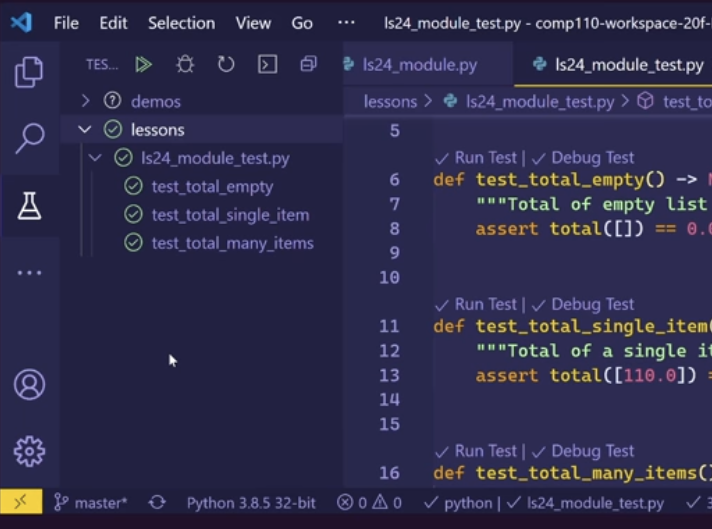
\includegraphics[scale = 0.6]{attachment/chapter_2/Scc082}
	\caption{Visual Studio Extenstion}
\end{figure}

\begin{itemize}
	\item Die Extension erkennt automatisch, welche Tests vorhanden sind. Dies unter der Voraussetzung, dass die Bezeichnungskonvension eingehalten werden.\footnote{
 \textit{Hinweis:} Wenn es zu einem syntaktischen Fehler in einem der Test-Skript kommt, können keine der Test ausgeführt werden.
}
\item Ebenso dürfe keine Syntax Fehler in keinem der Skripte in Repository/Workspace vorkommen. Tritt einer auf, kann kein Test durchgeführt werden. Mit dem Befehlt

\begin{lstlisting}[style=CMD, caption={Unit Test - Version 1; Skeleton-test.py}, captionpos=b]
python -m pytest Unit_Test/unit_test/test_Skeleton.py
\end{lstlisting}
 kann nachvollzogen werden, wo genau der Syntax Fehler entstanden ist.
\end{itemize}

\subsection{Test-Driven Programming}
\subsubsection{Konzept}
Ein Konzept bei der Implementierung von Test heißt \textit{Test-Driven Programming}. Dies bedeutet, dass bei der Entwicklung von Funktionen \footnote{
	 Synonym für Algorithmen oder Methoden)
} wird vor der ersten Entwicklung überlegt, wie die Tests für die Funktion aussehen können.

Diese Tests werden dabei als erstes implementiert. Dafür genügt es eine Skeleton Funktion zu schreiben. Zwei Fragen helfen bei der Weiterentwicklung der Funktion
\begin{itemize}
	\item What are some \textit{usual} input parameters? - Use Cases
	\item What are some valid but \textit{unusual} input parameters? - Edge Cases
\end{itemize}
Dies hilft sich zum Anfang Gedanken zu machen, was die Funktion können muss oder welche Situationen sie ausgesetzt ist. Wenn Funktionen if-else Statments besitzen, ist es ratsam, Testfunktionen zu schreiben, welche jeden Bestandteil der Funktion erreichen.


\subsubsection{Bsp.: Total Sum}
Der Aufbau von Unit Test wird an Hand von einem konkreten Beispielen erklärt. \footnote{
	\href{https://youtu.be/UMgxJvozR5A}{Introductry Tutorial on Unittest, Python, VSCode, Command-line}
}

\paragraph{Skeleton Funktion}
Um zu zeigen, welche Funktionalitäten zu berücksichtigen sind, wird eine \textit{Skeleton Funktion} geschrieben. Diese übernimmt nur die Aufgabe, dass die die Form und und Rahmenparameter einer Funktion besitzt, aber im innern nur den Rückgabewert bestimmt.

\begin{lstlisting}[style=python, caption={Skelton-Function - Version 1; Skeleton.py}, captionpos=b]
from typing import List

def total_sum(xs: List[float]) -> float:
    """
        Computes total sum of all float variables in list.
    """
    return -1.0
\end{lstlisting}

\paragraph{Test Case - 1}
Im nächsten Schritt soll überprüft werden, welche Anwendungsfälle die Funktion unterliegen kann. 

\begin{figure}[h]
	\centering
	\resizebox{0.2\textwidth}{!}{% Faktor zum Skalieren
		\begin{forest}
			for tree={
				font=\sffamily,
				grow'=0,
				folder indent=0.9em,
				folder icons,
				edge=densely dotted
			}
			[Application
			[..., is file]
			[test
				[Skeleton$\_$test.py, is file]
			]
			[..., is file]
			]
		\end{forest}
	}%
	\caption{Bsp.: Ordner Struktur Aufbau Testmodule}
\end{figure}

Dafür wird ein Unit Test im Verzeichnis \textit{test} angelegt. In jeden Unit Test befinden sich Test Funktionen. Diese benötigen den Prefix textit{test}$\_$.

\begin{lstlisting}[style=python, caption={Unit Test - Version 1; Skeleton-test.py}, captionpos=b]
from src.Skeleton import total
// TODO: Bilder ersetzen, mit eigenen aus der eigenen Durchführung
// Im Tutorial: lessons/ls_24_module_test.py
// Unit_Test/test_Skeleton.py ist das iOS Verzeichnis

def test_total_sum() -> None:
    """
        Testing the total sum function
    """
	assert total([]) == 0
	%
\end{lstlisting}

Der Ausdruck \textit{assert} sagt \textit{pytest}, dass hier eine Annahme vorliegt, welche überprüft werden soll. Im angegeben Beispiel wird der \textit{total} Funktion eine leere Liste übergeben. Es wird erwartet, dass die Funktion die Summe 0 zurückgibt.

Mit dem Command Befehl

\begin{lstlisting}[style=CMD, caption={Unit Test - Version 1; Skeleton-test.py}, captionpos=b]
python -m pytest Unit_Test/unit_test/test_Skeleton.py
\end{lstlisting}

wird \textit{pytest} auf das ausgewählte Modul angewandt.

\begin{figure}[H]
	\centering
	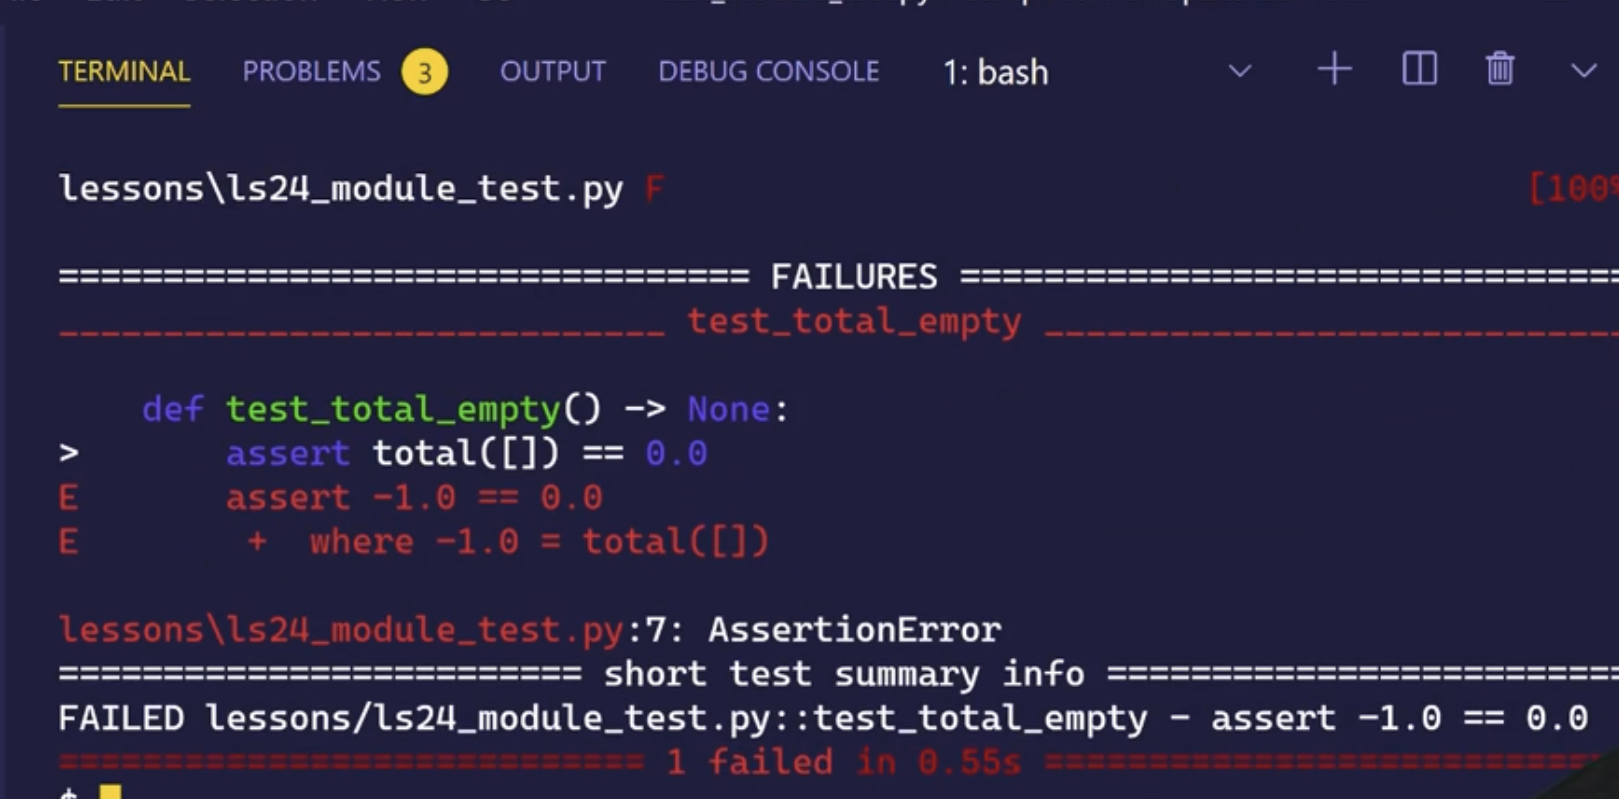
\includegraphics[scale = 0.6]{attachment/chapter_2/Scc085}
	\caption{pytest output - Version 1}
\end{figure}

Der Output gibt in diesem Fall wieder, dass es eine Fehler gab. 
\begin{itemize}
	\item In der ersten Zeile angegeben, in welchem Unit Test (Datei) es zum Fehler kam: \textit{lessons/ls-24-module-test.py}. Der Status $F$ hinter \textit{lessons/ls-24-module-test.py} gibt an, dass der Test gescheitert ist.
	\item Das Symbole $>$ zeigt an, in welcher Zeile es zu einem Problem kam. 
	\item Der Status $E$ zeigt an, dass es in der Zeile zu einem unerwartete Ausnahme kam. Diese wird angezeigt.
\end{itemize}

Der Status eines geprüften Zeile kann eins von drei Zuständen sein
\begin{description}
	\item[.] Der Test war erfolgreich. - The tests passed.
	\item[F] Der Test ist gescheitert. - The tests failed.
	\item[E] Der Test ist auf eine unerwartete Ausnahmen gestoßen. - The test raised an unexpected exeption. 
\end{description}

Der Fehler stammt daher, dass in der Funktion \textit{total-sum} der Rückgabewert auf $-1$ angegeben war.

\paragraph{Test Case - 2}
Würde der Rückgabewert auf $0.0$ gesetzt werden, würde auch der Test erfolgreich sein.

\begin{lstlisting}[style=python, caption={Skelton-Function - Version 2; Skeleton.py}, captionpos=b]
from typing import List

def total_sum(xs: List[float]) -> float:
    """
        Computes total sum of all float variables in list.
    """
    return 0.0
\end{lstlisting}

Der Output ist

\begin{figure}[H]
	\centering
	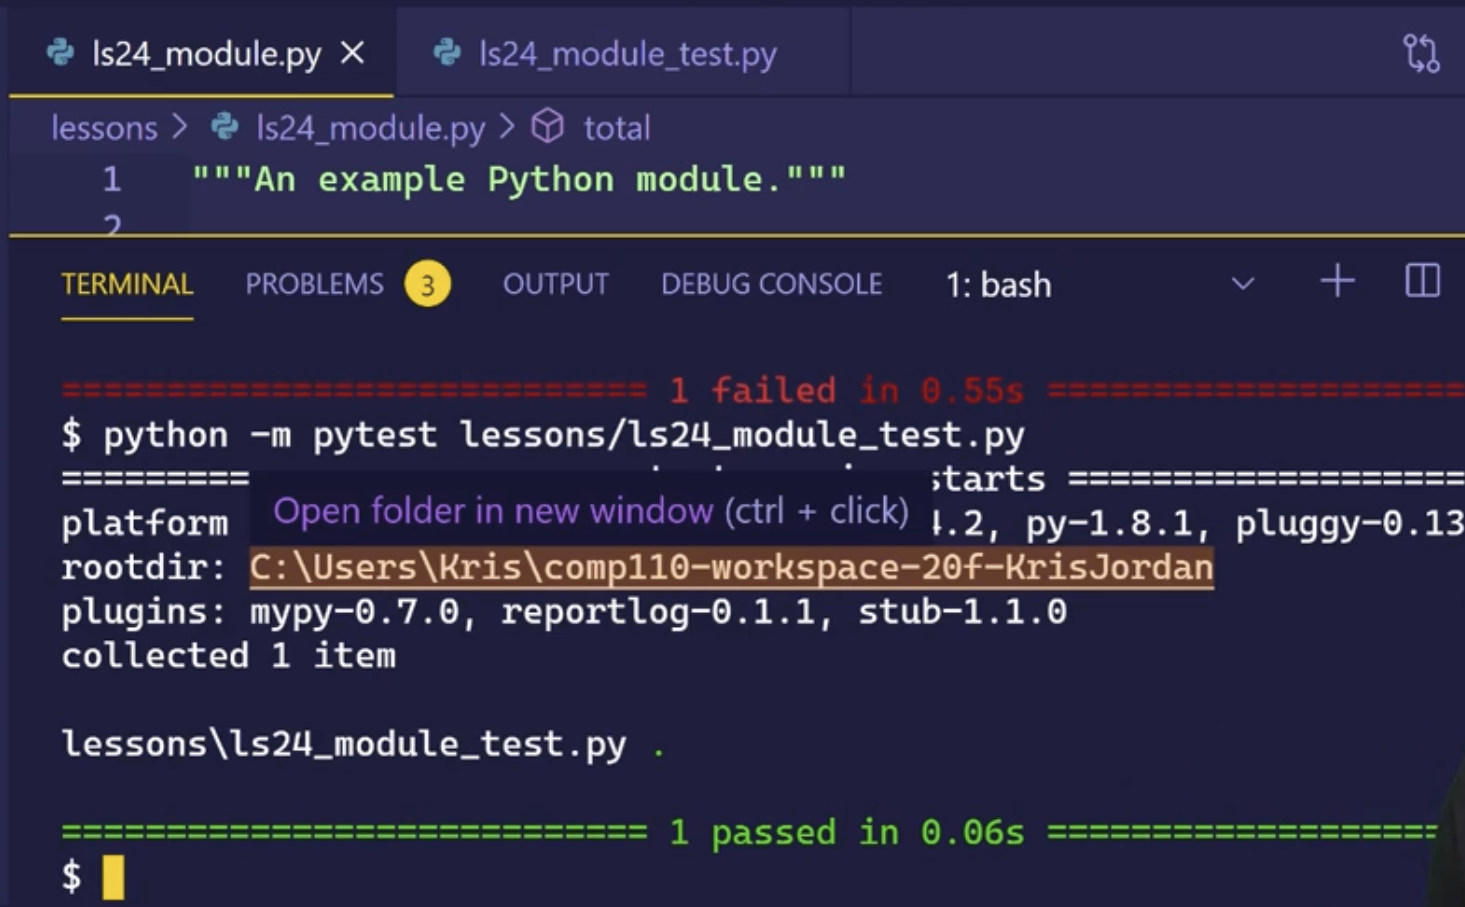
\includegraphics[scale = 0.6]{attachment/chapter_2/Scc086}
	\caption{pytest output - Version 2}
\end{figure}

Der Status $.$ hinter \textit{lessons/ls-24-module-test.py} gibt an, dass der Test erfolgreich durchgeführt wurde. Dies bedeutet auch, nur weil ein Test erfolgreich ist, muss die Funktion nicht ihre Aufgabe erfüllen. Daher ist es notwendig, den vollen Umfang einer Funktion zu überprüfen.

\paragraph{Test Case - 3}

\begin{lstlisting}[style=python, caption={Unit Test - Version 3; Skeleton-test.py}, captionpos=b]
from src.Skeleton import total
// TODO: Bilder ersetzen, mit eigenen aus der eigenen Durchführung
// Im Tutorial: lessons/ls_24_module_test.py
// Unit_Test/test_Skeleton.py ist das iOS Verzeichnis

def test_total_sum_empty() -> None:
    """
       Total sum of an empty list
    """
	assert total([]) == 0
	

def test_total_sum_single_item() -> None:
    """
       Total sum of a single item is the first item's value
    """
	assert total([110.0]) == 110.0

\end{lstlisting}
Es wurde ein zweites Testscenario hinzugefügt. Dies erweitert den zu prüfenden Rahmen der Funktion.

Wird der Test durchgeführt, wird angezeigt, dass ein Test erfolgreich und ein gescheitert ist.
\begin{figure}[H]
	\centering
	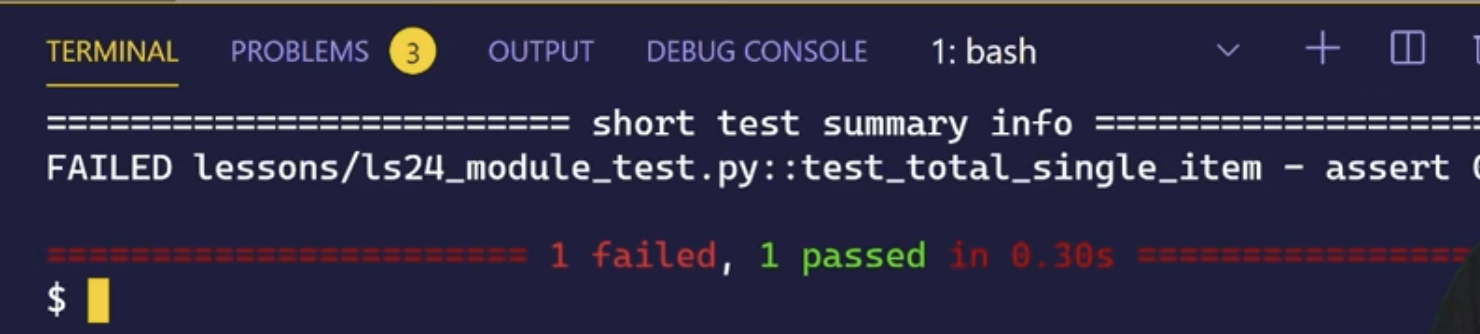
\includegraphics[scale = 0.6]{attachment/chapter_2/Scc087}
	\caption{pytest output summary - Version 3}
\end{figure}

In der Detailansicht kann nachgeschaut werden, wo und wie der Test gescheitert ist.

\begin{figure}[H]
	\centering
	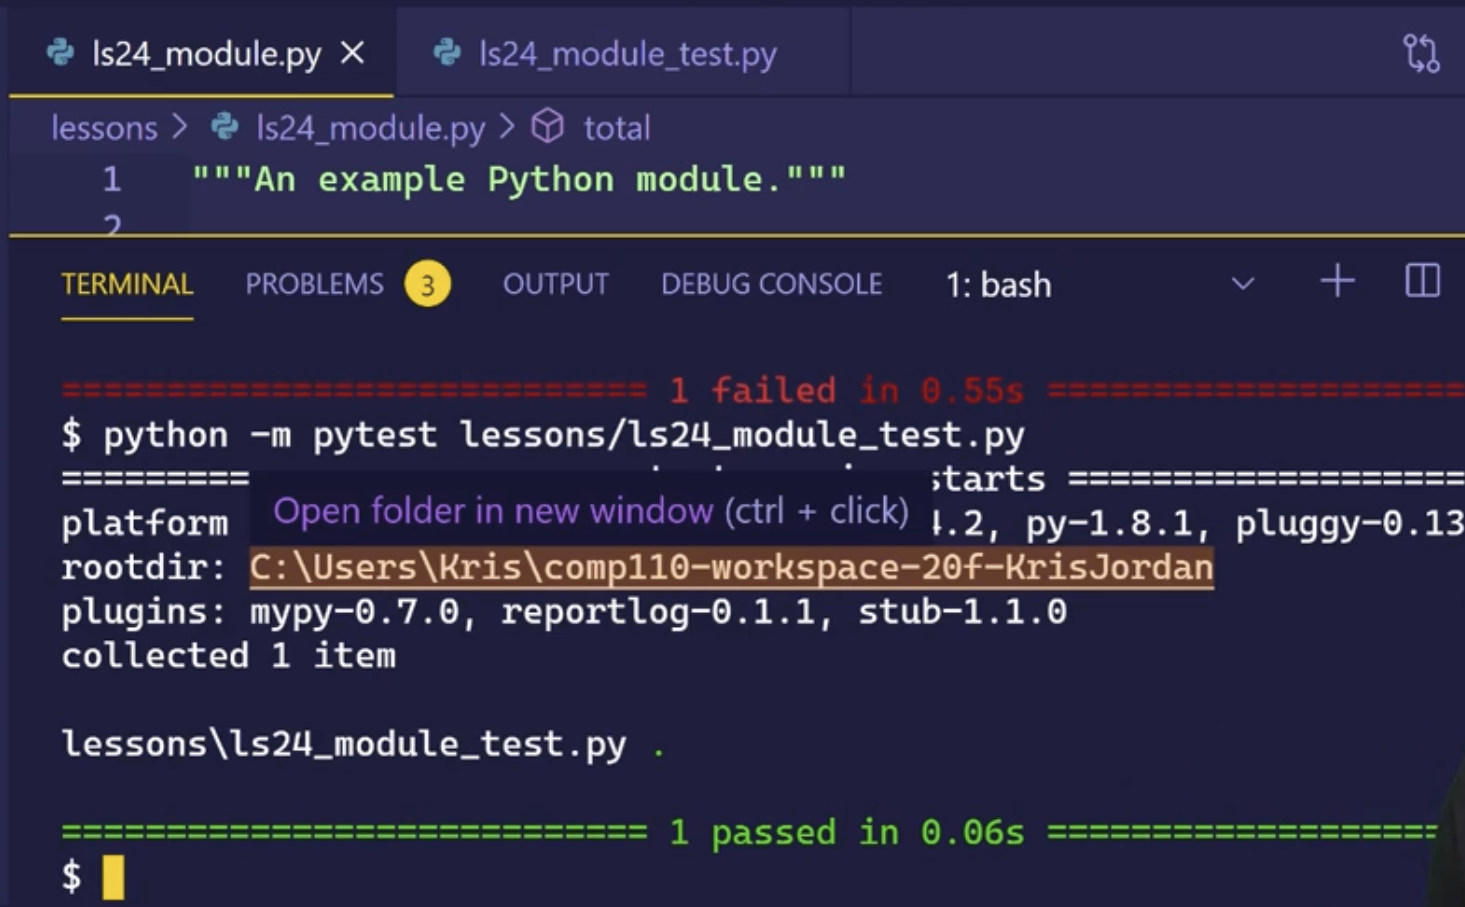
\includegraphics[scale = 0.6]{attachment/chapter_2/Scc086}
	\caption{pytest output detailiert - Version 2}
\end{figure}
Mit einer vollständigeren Funktion,

\begin{lstlisting}[style=python, caption={Skelton-Function - Version 4; Skeleton.py}, captionpos=b]
from typing import List

def total_sum(xs: List[float]) -> float:
    """
        Computes total sum of all float variables in list.
    """
    # Initial Value
    result = 0.0
    
    # Sum up all values in the list
    for x in xs:
    	result += x
    
    return result
\end{lstlisting}

wird der Test aus der Version 3 in beiden fällen erfolgreich sein.
\begin{figure}[H]
	\centering
	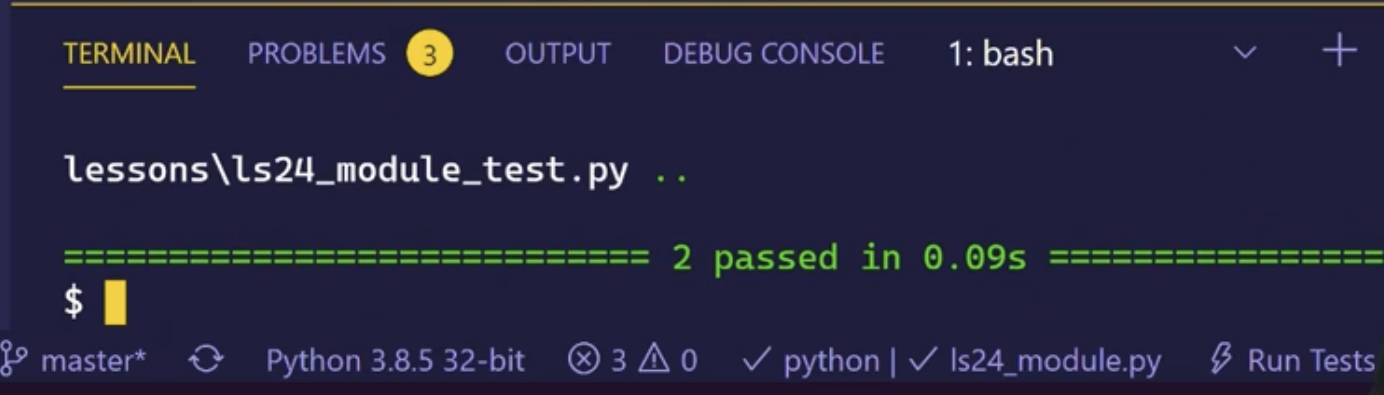
\includegraphics[scale = 0.6]{attachment/chapter_2/Scc089}
	\caption{pytest output summery - Version 4}
\end{figure}

Die beiden grünen Punkte hinter dem Testmodul zeigen, dass beide Test in dem Testmodul erfolgreich durchgelaufen sind.	

\subsubsection{Bsp.: Join}

Die Funktion \textit{join} soll eine Liste von Zahlen durch eine gegebenes Trennzeichen als String wieder geben.
In diesem Fall wurde keine Funktion \textit{join} erstellt, sondern nur die Test-Funktionen erstellt.
\begin{figure}[H]
	\centering
	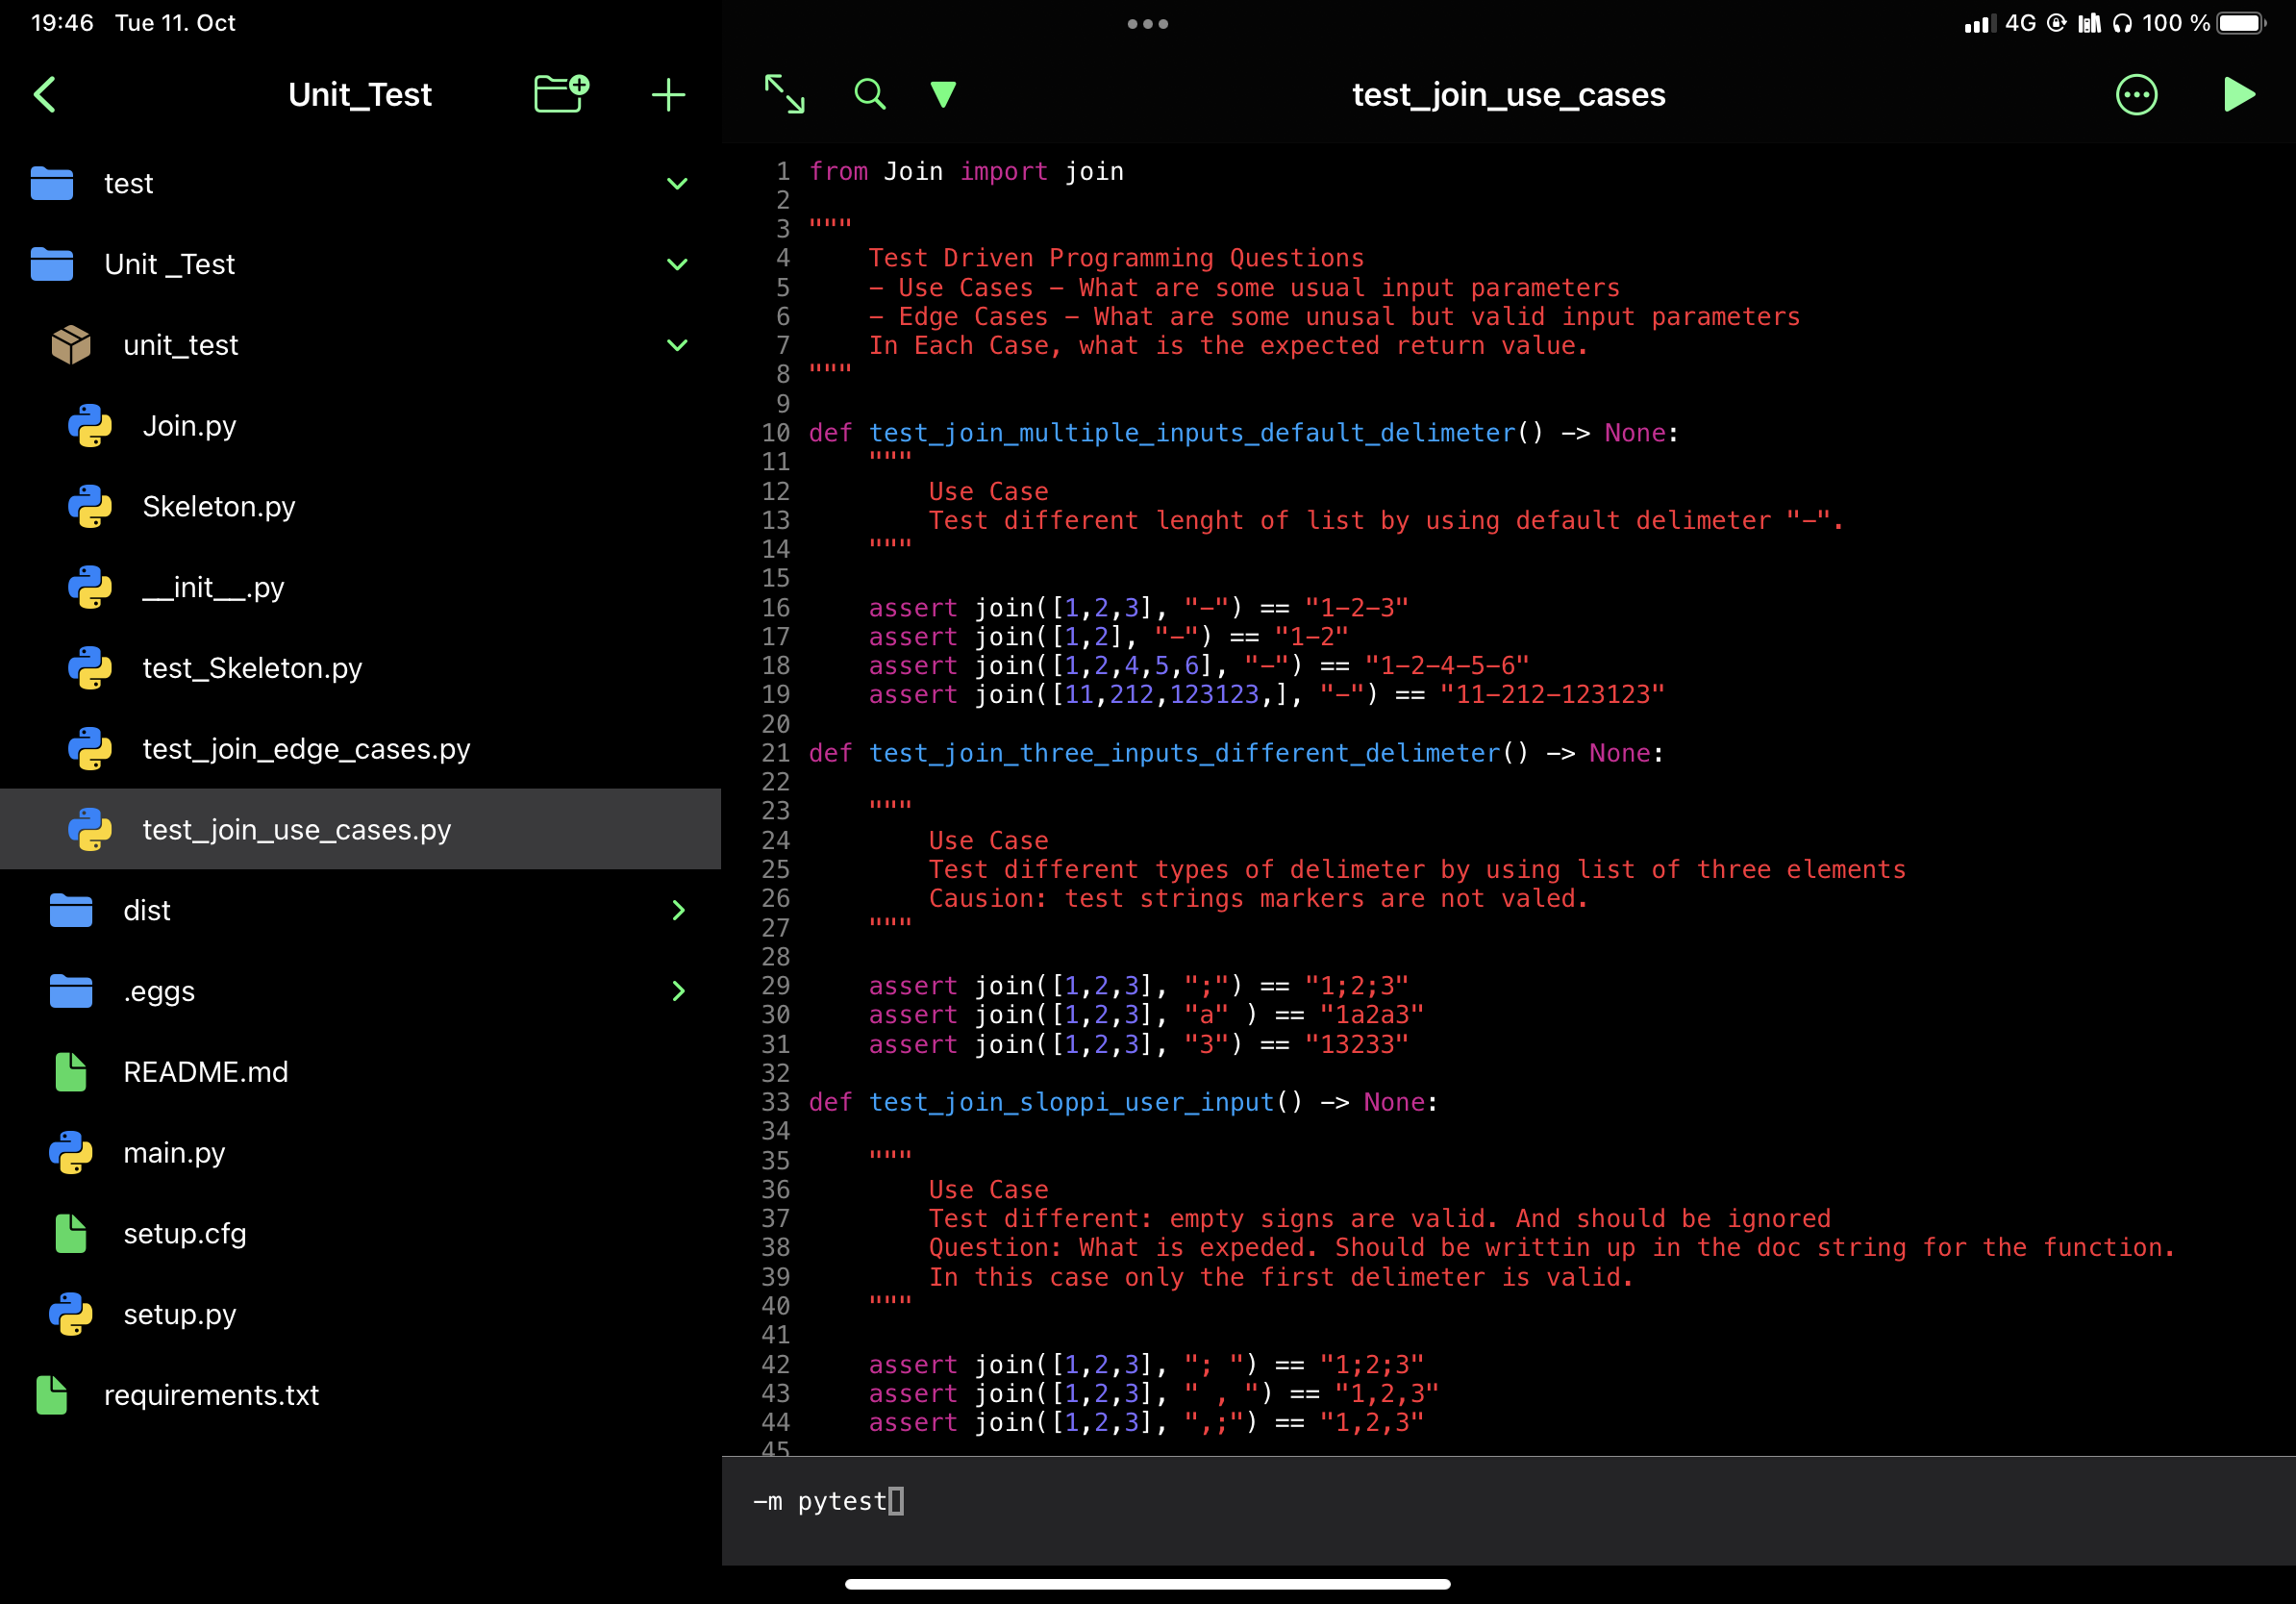
\includegraphics[scale = 0.6]{attachment/chapter_2/Scc090}
	\caption{Use Cases - Join}
\end{figure}

\begin{figure}[H]
	\centering
	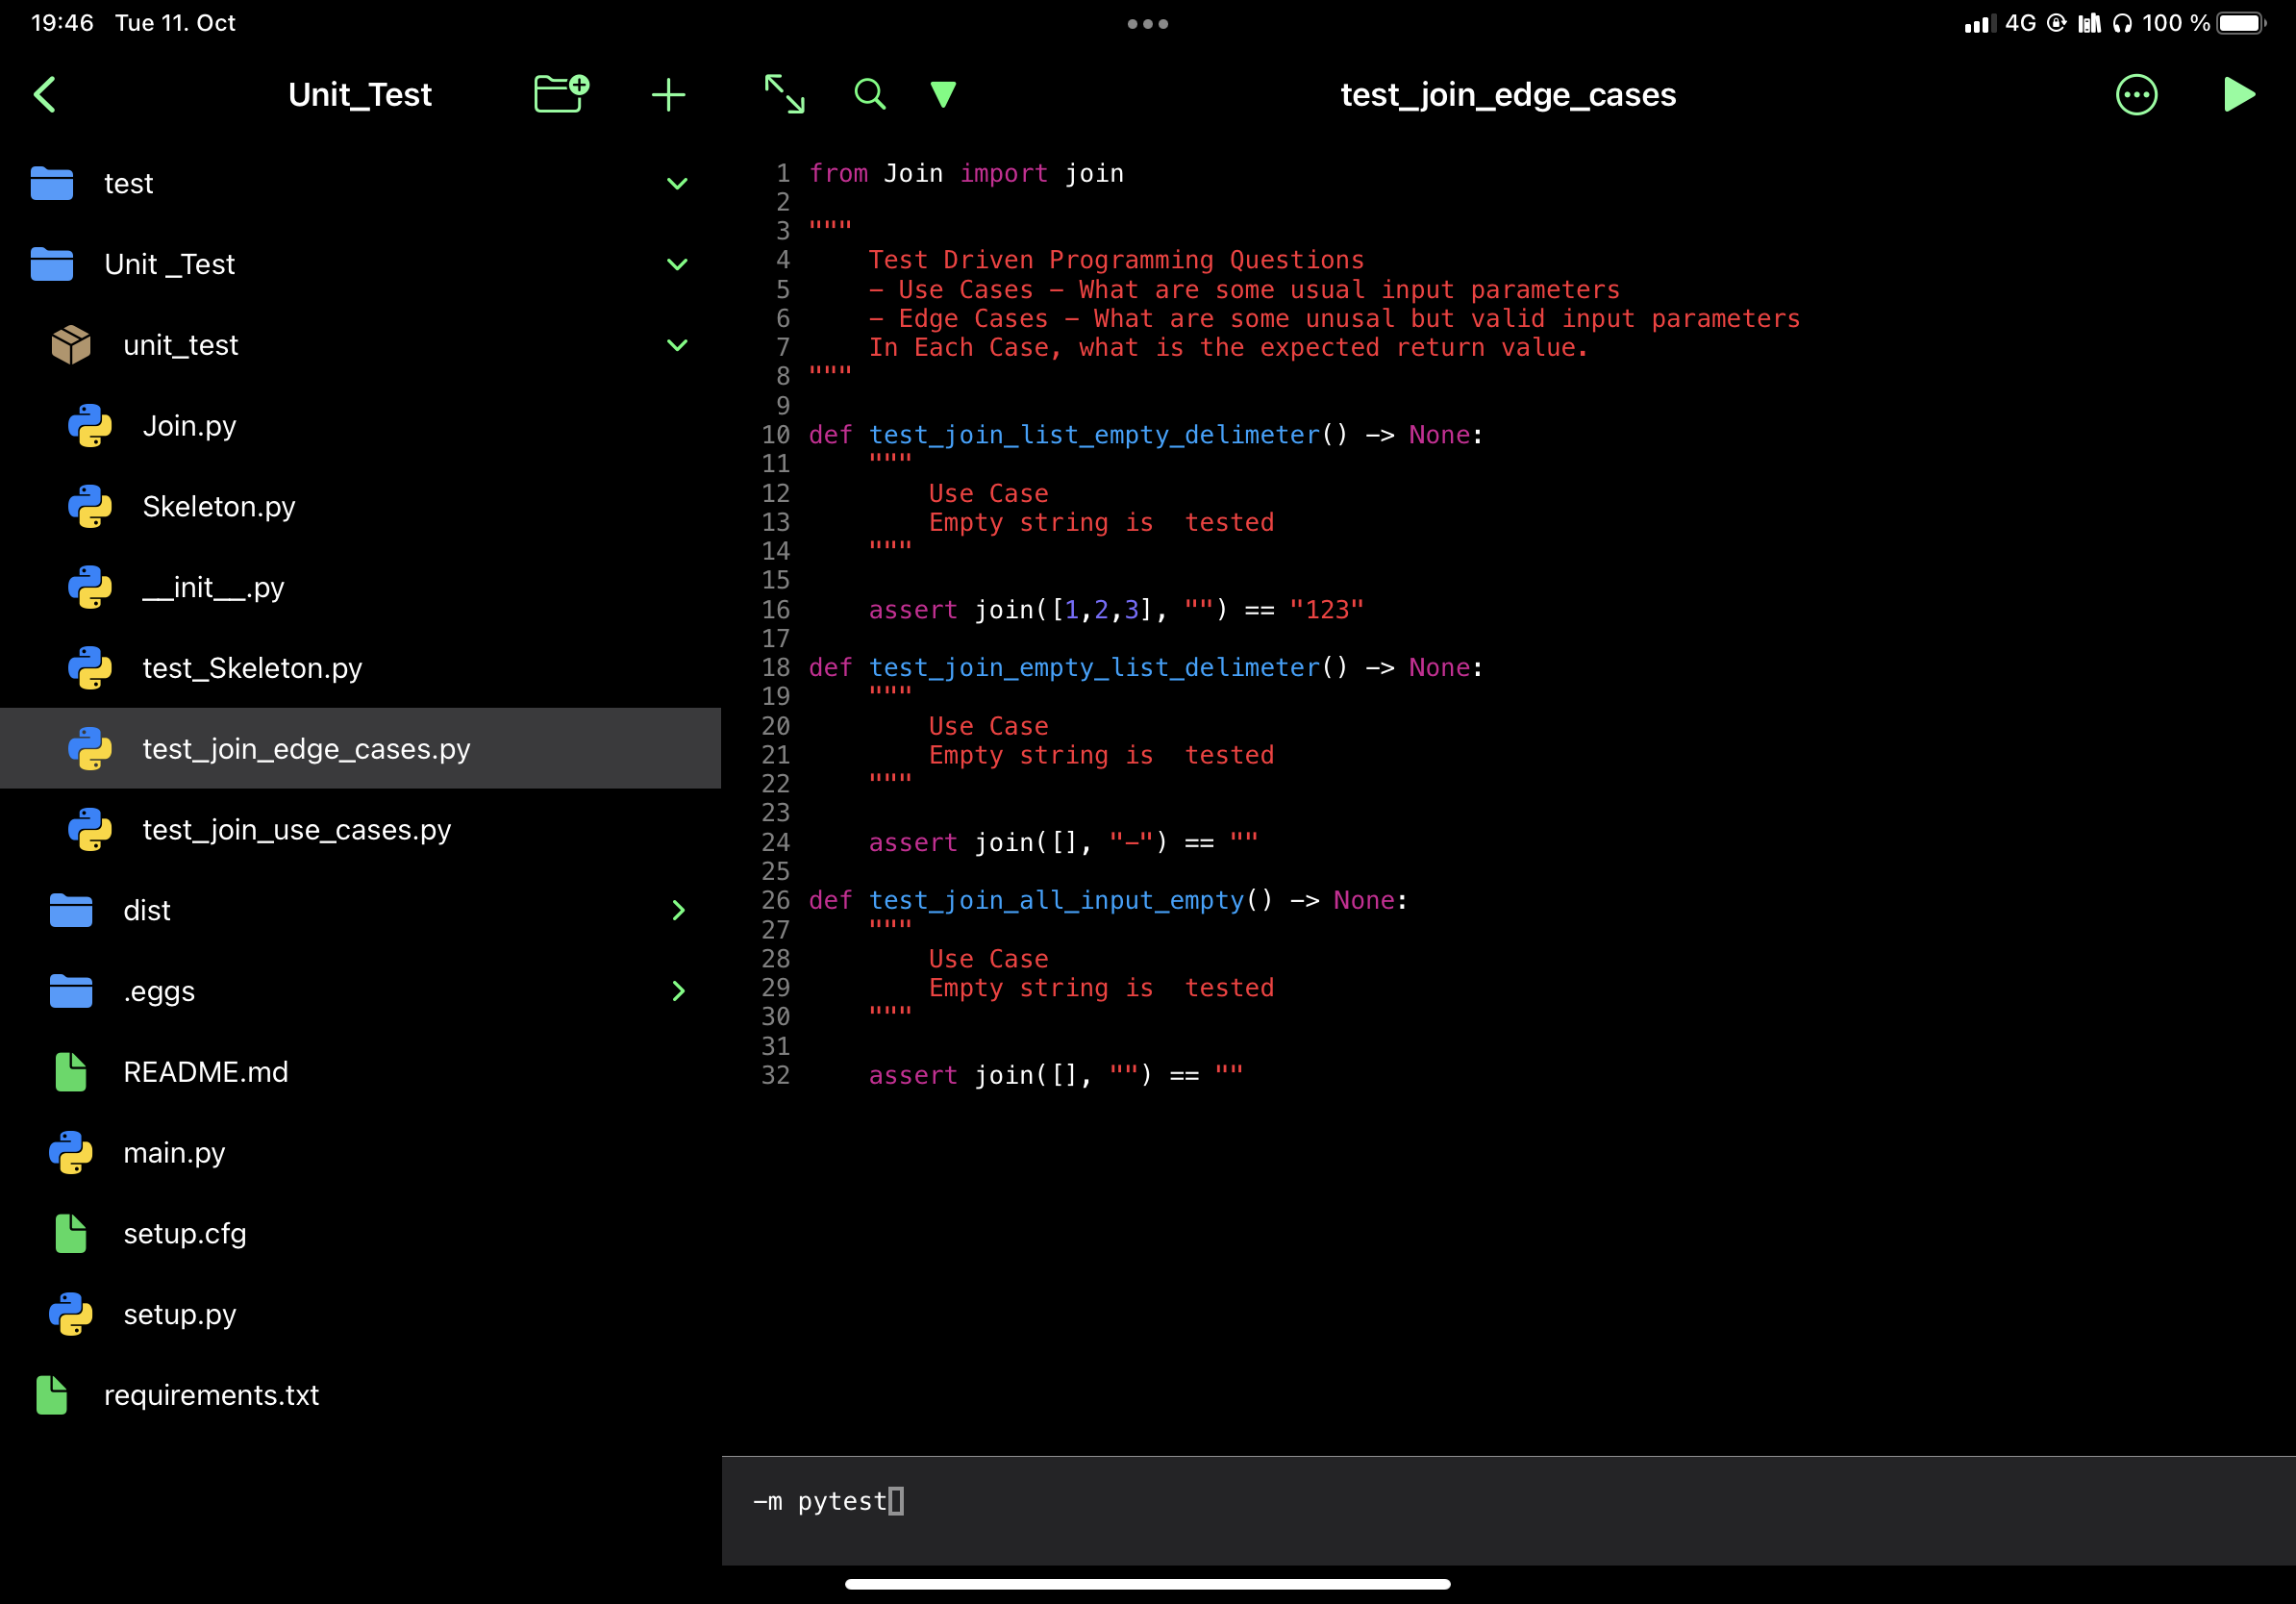
\includegraphics[scale = 0.6]{attachment/chapter_2/Scc091}
	\caption{Edge Cases - Join}
\end{figure}

\subsubsection{Other Topics}
Hier nicht im Detail behandelt, sind
\begin{itemize}
	\item pytest.fixers 
	\begin{lstlisting}[style=python]
# test_format_data.py
import pytest

@pytest.fixture
def example_people_data():
    return [
        {
            "given_name": "Alfonsa",
            "family_name": "Ruiz",
            "title": "Senior Software Engineer",
        },
        {
            "given_name": "Sayid",
            "family_name": "Khan",
            "title": "Project Manager",
        },
    ]

# ...
	\end{lstlisting}
	\item 
\end{itemize} 

\subsection{Coverage Bibliothek}
\subsubsection{Konfiguration - Directory}
Unter \ref{par:Setup pyprojekt.toml} ist die Einbindung der Bibliothek zu finden. 

\begin{lstlisting}[style=Config, caption={Beispiel pyproject.toml; Slapping pytest config}, captionpos=b]
...
[tool.pytest.ini_options]
addopts = "--cov=slapping"
testpaths = [
	"tests",
]
\end{lstlisting}
Der Befehl \textit{--cov=} gibt an in welchem Verzeichnis pytest-cov angewandt werden soll. Dies kann auch über die Kommandozeile übergeben werden.

\begin{lstlisting}[style=CMD, caption={Bsp. Befehl zum Ausführen von pytest cov}, captionpos=b]
python -m pytest --cov=myproj tests/	
\end{lstlisting}

Wir vom aktuellen Verzeichnis gestestet werden, so wird \textit{--cov .} benötigt

\begin{lstlisting}[style=CMD, caption={Bsp. Befehl zum Ausführen von pytest cov - Same directory}, captionpos=b]
python -m pytest --cov .
\end{lstlisting}

Ist der Vermerk auf die Anwendung der Coverage Bibliothek in der Konfigurations pyproject.toml hinterlegt, reicht die Ausführung

\begin{lstlisting}[style=CMD, caption={Bsp. Befehl zum Ausführen von pytest und cov, config erfüllt}, captionpos=b]
python -m pytest
\end{lstlisting}

\subsubsection{Konfiguration - HTML Report}
Um einen Report auszugeben, wird \textit{--cov-report} benötigt. Es gibt verschiedenen Formate. Hier wird das Format \gls{HTML} benötigt.

\begin{lstlisting}[style=CMD, caption={Bsp. Befehl zum Ausführen von pytest cov}, captionpos=b]
python -m pytest --cov=myproj tests/ --cov-report html
\end{lstlisting}

In der Konfigurationsdatei wird dies als Teil des \textit{apdopts} String mit übergeben.

\begin{lstlisting}[style=Config, caption={Beispiel pyproject.toml; Slapping pytest config}, captionpos=b]
...
[tool.pytest.ini_options]
addopts = "--cov-report html --cov=slapping"
testpaths = [
	"tests",
]
\end{lstlisting}

\subsubsection{Anwendung}
	Die Coverage Bibliothek hat das Ziel, detailliert wiederzugeben, wieviel der zu testenden Funktionen und Dateien wirklich kontrolliert wurden. 

\begin{figure}[H]
	\centering
	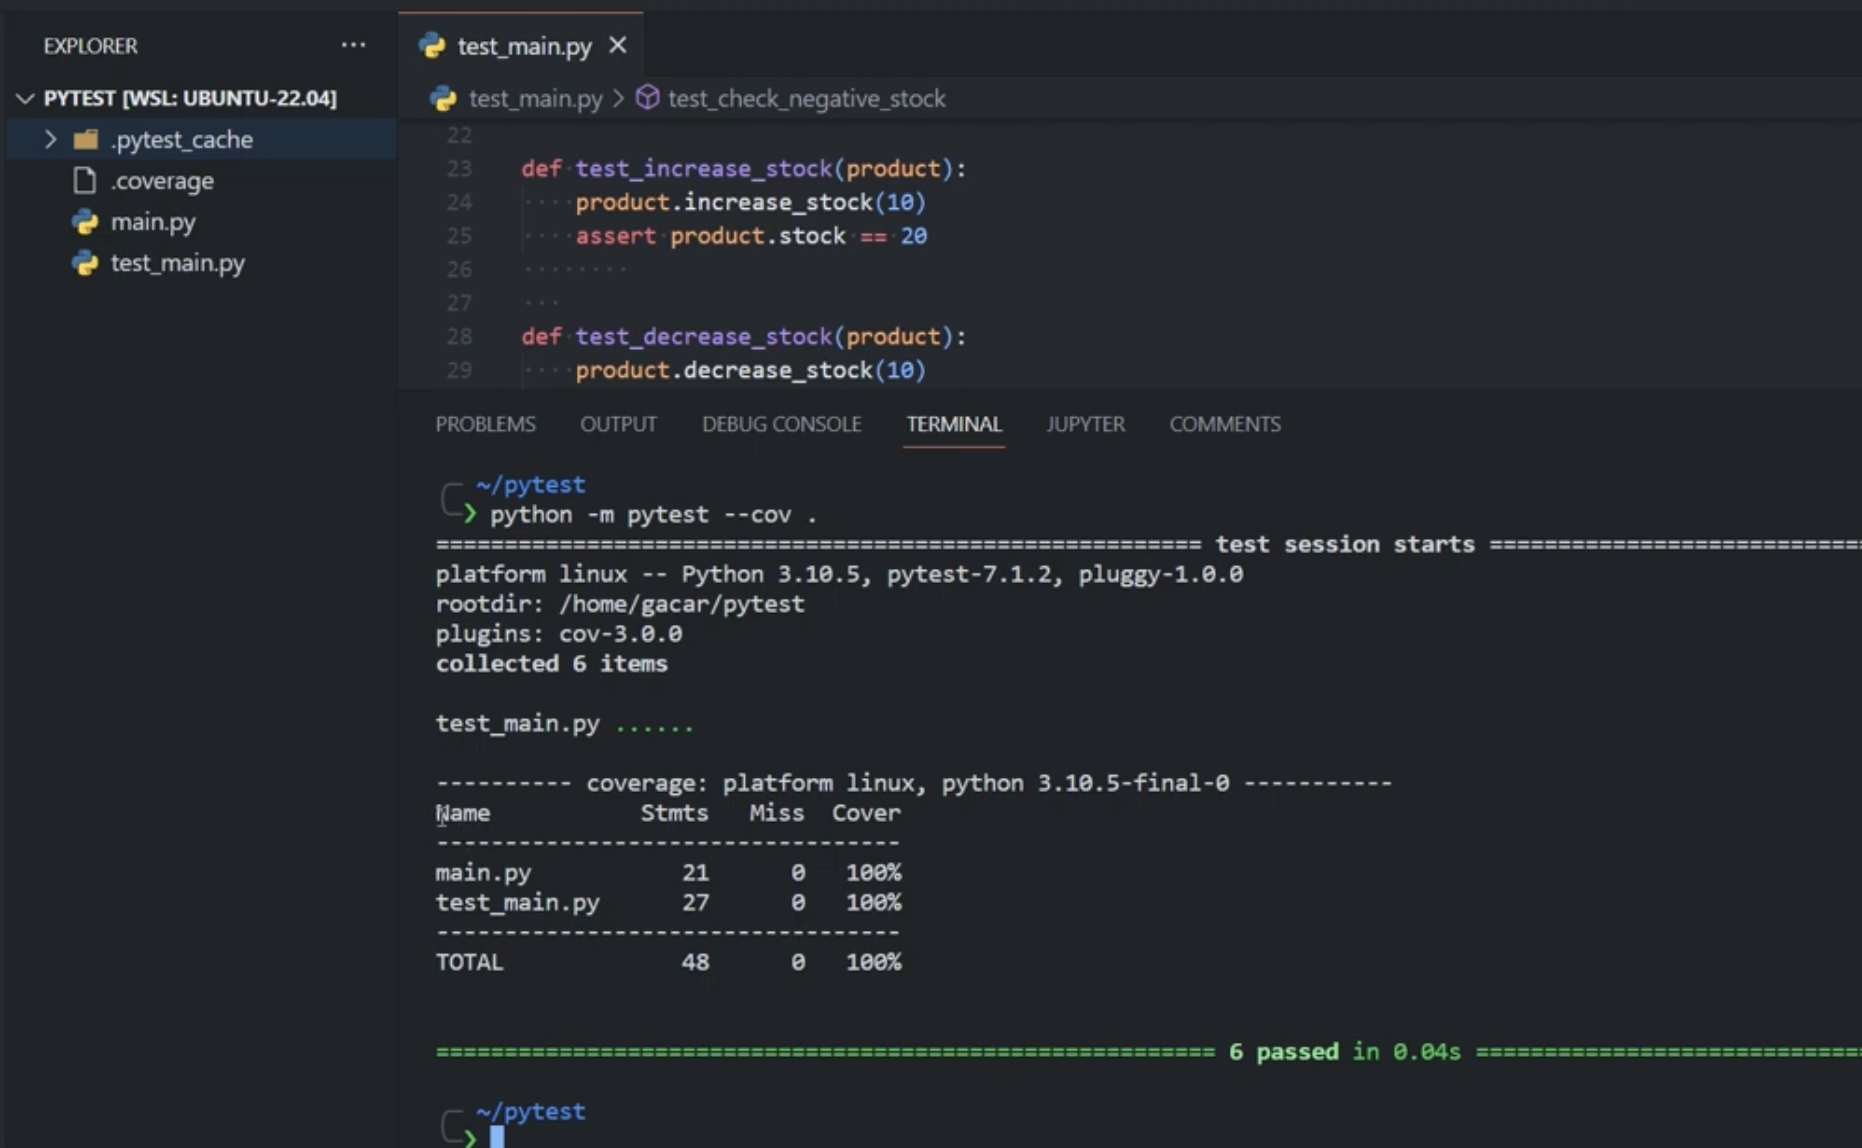
\includegraphics[scale = 0.6]{attachment/chapter_2/Scc092}
	\caption{Bsp. Report pytest cov}
\end{figure}

In dieser Ansicht wird mehr Informationen angeben, welche helfen sollen, einzusehen, wie hoch der Anteil der Skripte ist, welche von den Tests erreicht werden.
\begin{itemize}
	\item Die sechs grünen Punkte geben an, dass die sechs Testfunktionen in dem Testmodul erfolgreich getestet wurden.
	\begin{figure}[H]
	\centering
	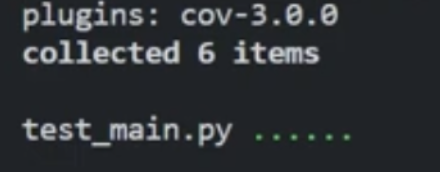
\includegraphics[scale = 0.6]{attachment/chapter_2/Scc093}
	\caption{Bsp. Report pytest cov - Testfunktionen}
\end{figure}
	\item \textit{Smtp} - Statements in the file,  zeigt, wie viele zu überprüfende Aussagen es in jeder Datei gibt. In der nächsten Spalte wird angezeigt, wieviele davon nicht erreicht wurden.
	\begin{figure}[H]
	\centering
	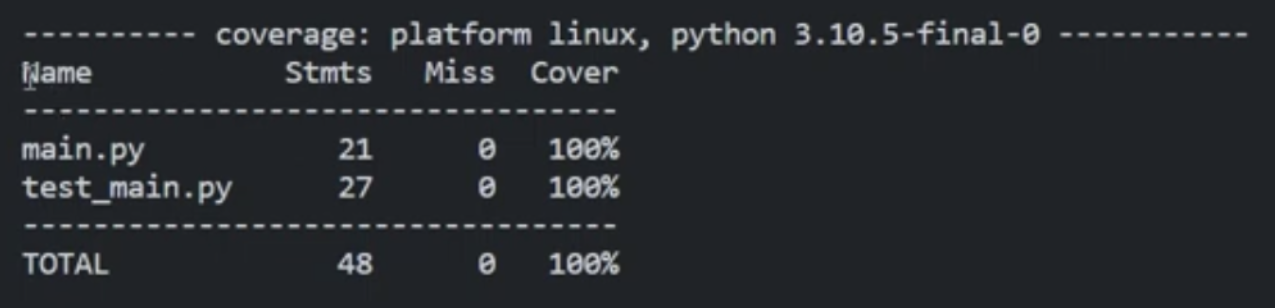
\includegraphics[scale = 0.6]{attachment/chapter_2/Scc094}
	\caption{Bsp. Report pytest cov - Coverage Übersicht}
\end{figure}
\end{itemize}

Mit der Option \textit{--cov-report html} wird das Verzeichnis \textbf{htmlcov} abgelegt.

\begin{figure}[h]
	\centering
	\resizebox{0.2\textwidth}{!}{% Faktor zum Skalieren
		\begin{forest}
			for tree={
				font=\sffamily,
				grow'=0,
				folder indent=0.9em,
				folder icons,
				edge=densely dotted
			}
			[Application
			[..., is file]
			[test
				[Unit1$\_$test.py, is file]
				[Unit2$\_$test.py, is file]
			]
			[htmlcov/]
			[scr/]
			[..., is file]
			]
		\end{forest}
	}%
	\caption{Bsp.: Coverage Report - htmlcov}
\end{figure}

In dem Verzeichnis ist die Datei \textit{index.html} enthalten.
\begin{figure}[H]
	\centering
	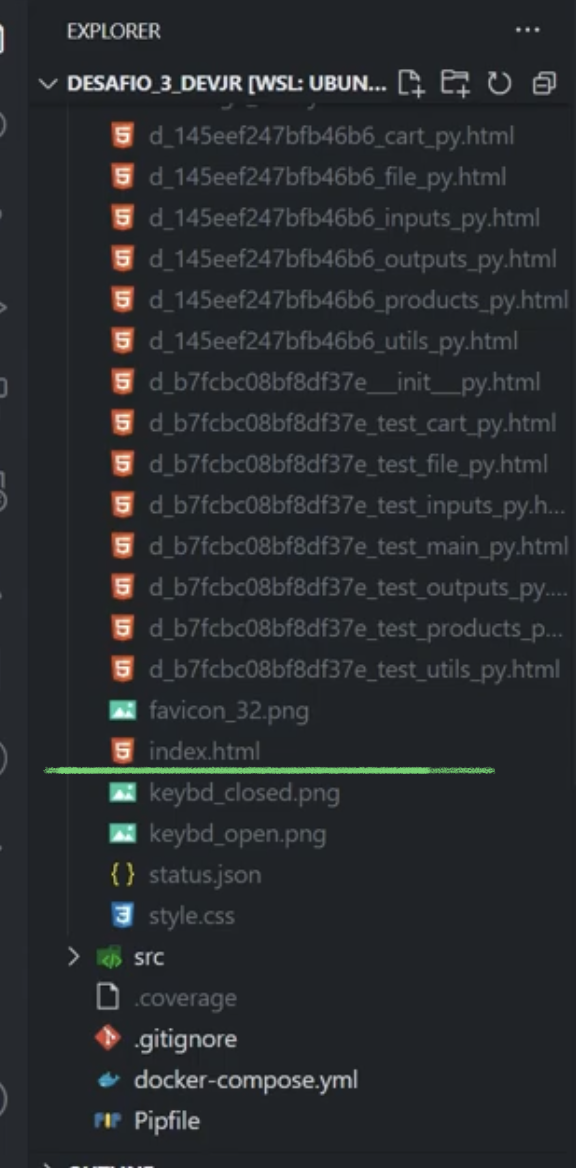
\includegraphics[scale = 0.6]{attachment/chapter_2/Scc095}
	\caption{Bsp. Report pytest cov report - index file}
\end{figure}
Diese gibt einen Überblick über alle getesteten Skripte.

\begin{figure}[H]
	\centering
	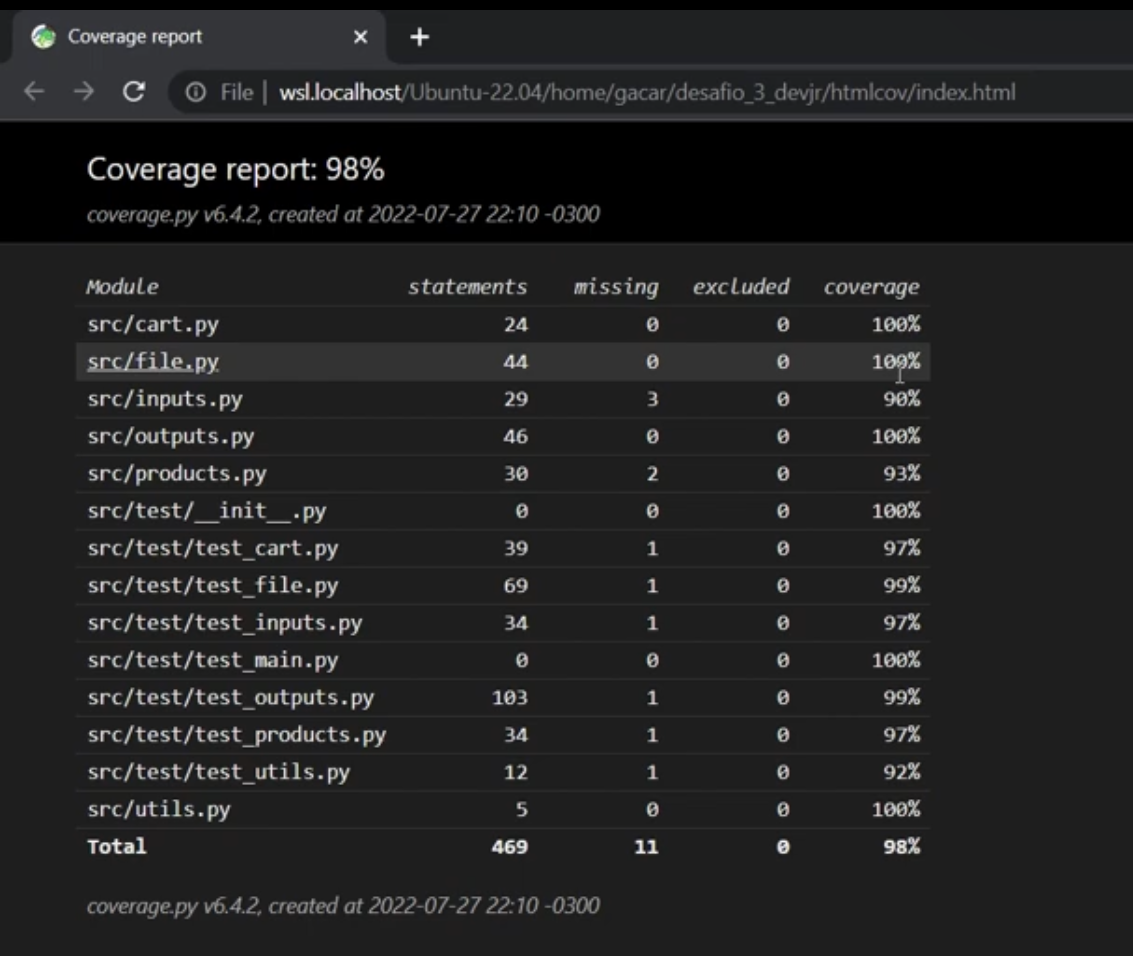
\includegraphics[scale = 0.6]{attachment/chapter_2/Scc096}
	\caption{Bsp. Report pytest cov report index - Übersicht}
\end{figure}
Hinter jedem Skript liegt eine Auswertung, welche genau zeigt, welche Code Zeilen erreicht und welche nicht erreicht werden.
\begin{figure}[H]
	\centering
	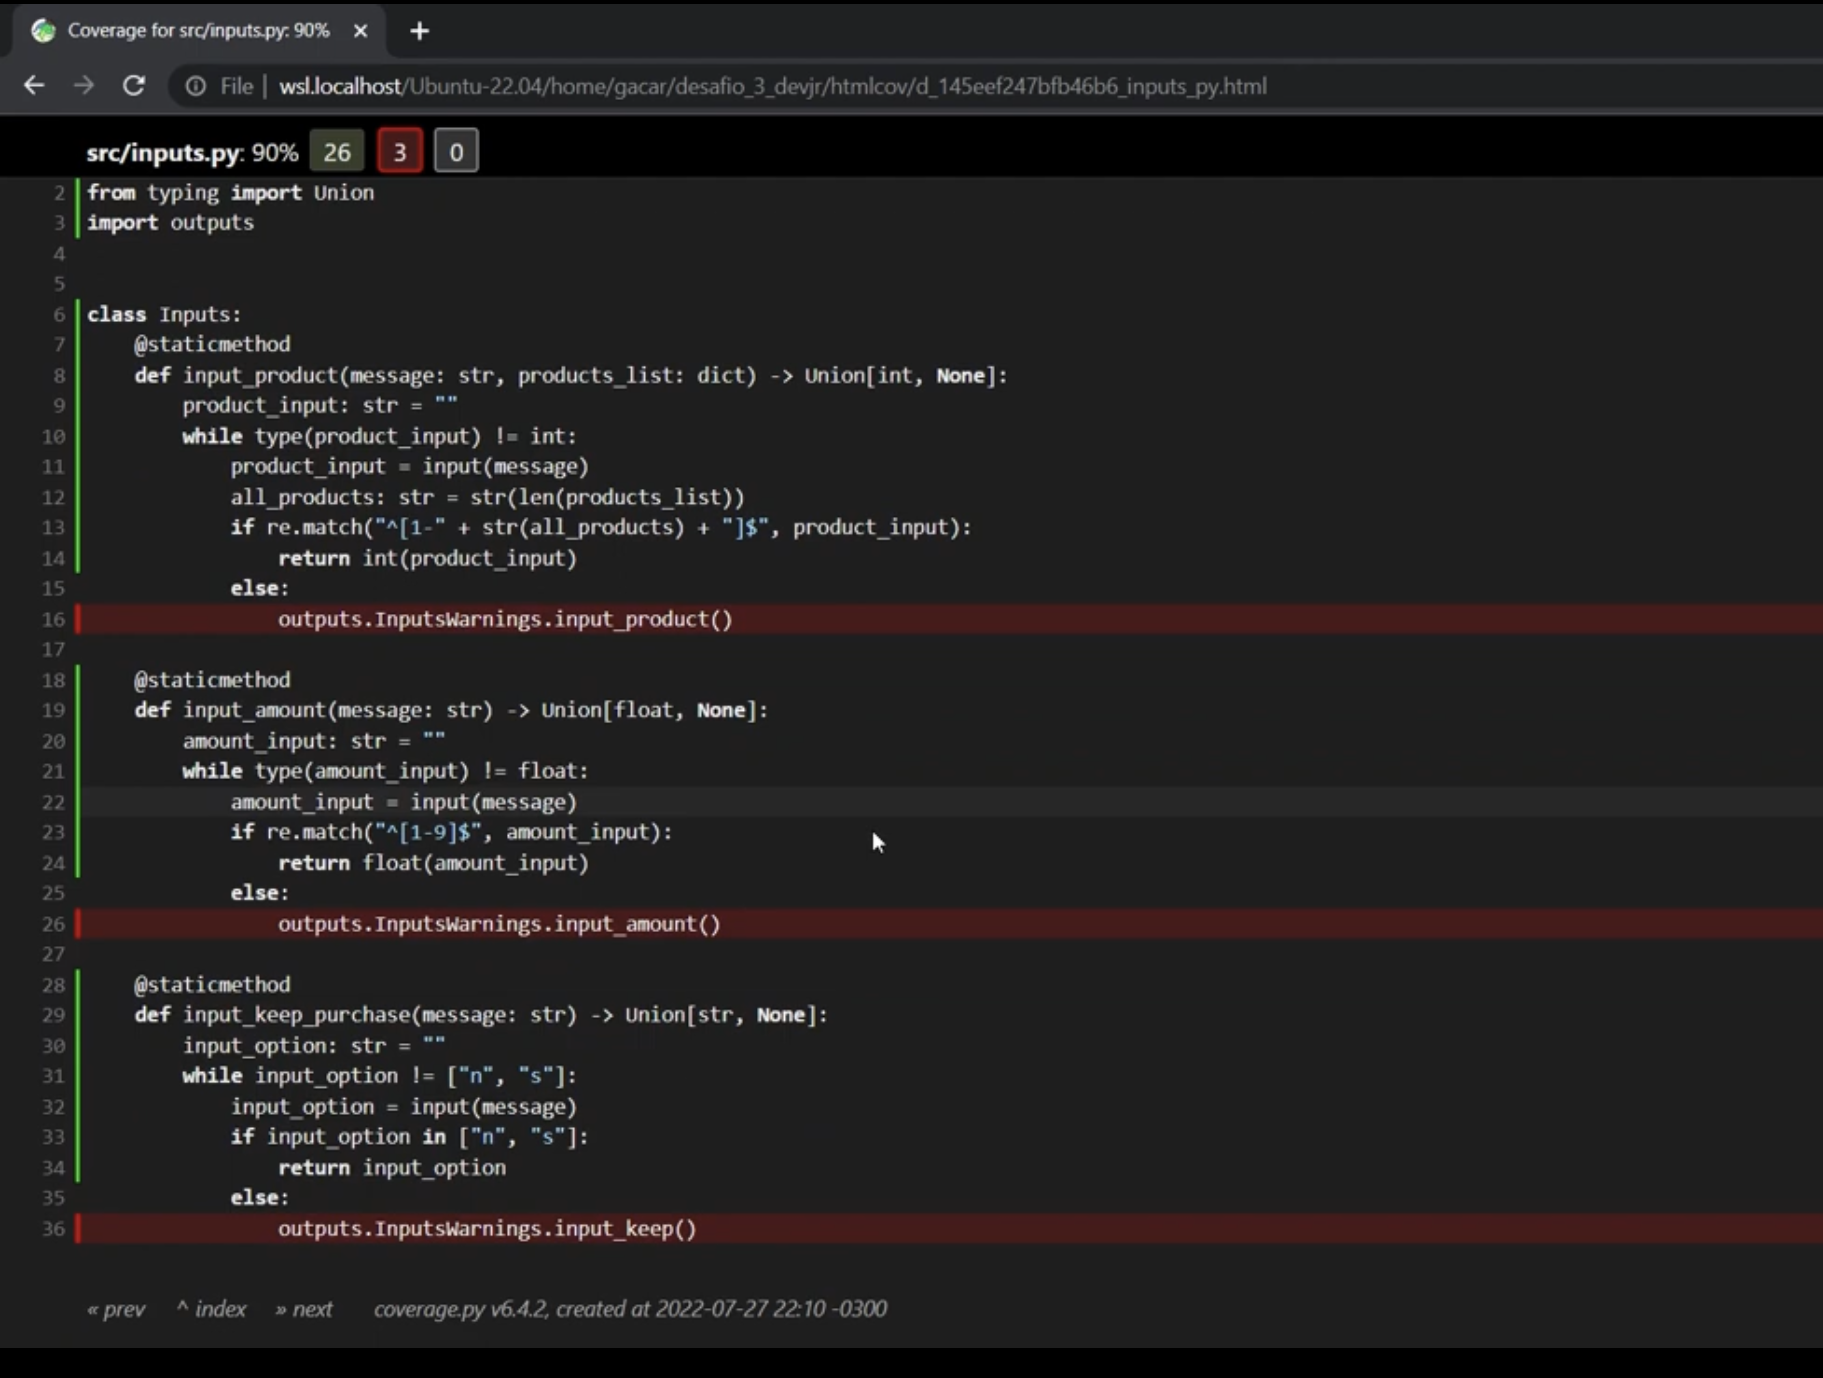
\includegraphics[scale = 0.6]{attachment/chapter_2/Scc097}
	\caption{Bsp. Report pytest cov report index - Einzelauswertung}
\end{figure}

\subsection{Fixtures}

\subsubsection{Fixture Function}
Ein Deklarator \textit{Fixture} hilf die notwendigen Vorarbeiten für den Test zu übernehmen. Dabei werden Definitionen und Settings einheitlich für die Tests geteilt. 
Es wird bis auf den Test alles für den Test notwendige darin festgehalten. Wenn \textit{pytest} die Testfunktionen ausführt, dann wird überprüft, wenn die Funktion Parameter übergeben bekommen hat, ob diese als Fixtures deklariert sind. Sind sie es, dann wird der Fixtures ausgeführt.

\begin{lstlisting}[style=python, caption={Beispiel pyproject.toml; Slapping pytest config}, captionpos=b]
import pytest


class Fruit:
    def __init__(self, name):
        self.name = name

    def __eq__(self, other):
        return self.name == other.name


@pytest.fixture
def my_fruit():
    return Fruit("apple")


@pytest.fixture
def fruit_basket(my_fruit):
    return [Fruit("banana"), my_fruit]


def test_my_fruit_in_basket(my_fruit, fruit_basket):
    assert my_fruit in fruit_basket
\end{lstlisting}

\begin{itemize}
	\item Um Fixtures anders zu organisieren, wird \textit{conftext.py} erstellt, welches die Fixtures behinhaltet. In diese Datei werden alle Fixture hineingeladen, sodass pytest weiß, welche Fixtures es gibt. Dies bedeutet, dass Fixtures in mehren Modulen abglegt werden kann.
	\item Fixtures haben den Vorteil gegenüber Globale Variablen, dass sie bei jeden Aufruf neu gelesen werden, ob im Testprozess geändert zu werden.
\end{itemize}
\paragraph{Scope Option}
Dies Option erlaubt, einen Fixtures über eine festgelegten Aktionsraum unverändert zu lassen. 

\begin{lstlisting}[style=Config, caption={Beispiel pyproject.toml; Slapping pytest config}, captionpos=b]
...
@pytest.fixture(scope="session")
def spark(request):
	spark = {
		Sparksession
		.builder
		.appname("pytest_local_connection)
		...
	}
	
	request.addfinalizer(lambda: spark.stop())
	# Am Ende der test session, 
	# spark session wird geschlossen.
    return spark
\end{lstlisting}

Mit der Option scope = $"$session$"$ wird die Spark Session für den Lauf des kompletten Test erstellt. Diese bedeutet, jeder Test greift auf die lokale Spark Session zu. Diese verhindert, dass eine Spark Cluster aufgebaut wird und die meiste Zeit des Test mit dem Auf- und Abbau von Spark Session beschäftigt ist.\\

Der übergeben Parameter \textit{request} übergibt Werte aus der Test-Session dem Fixtures.


\subsubsection{mark.parametrize} 
Unter Parametrization wird hier verstanden, eine Prozess abhängig von Parametern zu machen, welche unabhängig gleich von dem Prozess verwendet werden. pytest ermöglicht für verschiedenen Sachverhalte zu parametrizieren. Mit \textit{mark.parametrize} können mehrer Argumente in einem  Tupel hinterlegt werden.
%TODO: Test
% Test how the it works with multiple arguments in a tupel.
\begin{lstlisting}[style=python, caption={Example Parametrizing test function with 2 variables}, captionpos=b]
...
@pytest.mark.parametrize(
	"""
	Unclear: how multiple input arguments can be given.
	Example: "var_1, var_2, ..., result", [(var_1_value_1, var_2_value_1, ..., result_1), ... ]
	or "var_n, result", [((var_1_value_1, var_2_value_1, ... ), result_1), ... ]
	"""
	"test_input, expected",	
	[
		(<input>,<output>),
		(<input>,<output>),
		...
	]
)
...
\end{lstlisting}

Argumente für eine Testfunktion können mit
\begin{lstlisting}[style=python, caption={Example Parametrizing test function with 2 variables}, captionpos=b]
...
@pytest.mark.parametrize(
	"test_input, expected",	
	[
		(<input>,<output>),
		(<input>,<output>),
		...
	]
)
...
\end{lstlisting}
parametriziert werden. 

\begin{comment}	
\begin{lstlisting}[style=python, caption={Bsp.: Parametrizing test function pytest - Part I}, captionpos=b]
		from Join import join
		
		"""
		Test Driven Programming Questions
		- Use Cases - What are some usual input parameters
		- Edge Cases - What are some unusal but valid input parameters
		In Each Case, what is the expected return value.
	
		"""
			input = 	[
			([1,2,4], "-", "1-2-3"),
			([1,2], "-", "1-2"),
			([1,2,4,5,6], "-", "1-2-4-5-6"),
			([11,212,123123], "-", "11-212-123123"),
			]
			
		@pytest.mark.paramatize("test_input_numbers, test_input_delimeter, expection", input)
	# Ich vermute, dass es recht simple ist, es wird jedes Tupel getest
	
\end{lstlisting}
\end{comment}

\begin{lstlisting}[style=python, caption={Bsp.: Parametrizing test function pytest - Part II}, captionpos=b]
	# The rest must be looked up in the Latex comment section. Coun't be compiled.
	
	def test_join_multiple_inputs_default_delimeter(test_input_numbers, test_input_delimeter,expection) -> None:
	"""
	Use Case
	Test different lenght of list by using default delimeter "-".
	"""
	
	assert join(test_input_delimeter, test_input_delimeter) == expection
\end{lstlisting}

Die Test-Funktion überprüft jedes übergebene Tupel. Jedes Tupel generiert somit einen Test.
%TODO: Test
% Dies muss getestet werden: @pytest.mark.paramatize
% ob die die parameterizierte Argumente auch so verhalten


\subsection{Marking}
\subsubsection{Skip a test}
Mit dem Marker \textit{@pytest.mark.skip()} wird die nachfolgende Test-Funktion gekennzeichnet, dass sie übersprungen wird. Hindergrund kann sein, dass die Funktion noch nicht implementiert wurde. Über die Test-Driven Prinzip gleich schon ein Test gelegt wird.

\begin{lstlisting}[style=python, caption={Bsp.: Skip a test function}, captionpos=b]
	...
	@pytest.mark.skip(reason="regex is no implemented yet")
	def test_function():
	...
\end{lstlisting}

\subsubsection{Expect an error}
Wenn eine Test Funktion eine Fehler hervorrufen soll, dann kann die mit \textit{pytest.raises()} überprüft werden.

\begin{lstlisting}[style=python, caption={Bsp.: Expect an erro a test function}, captionpos=b]
...
def test_invalid_value():
	with pytest.raised(ValueError):
		slap_man(LikeState.empty, "x")
...
\end{lstlisting}
Die Testfunktion wird jetzt als gescheitert betrachtet, wenn kein Fehler aufgetreten ist.

\subsubsection{Expect an Fail}
\begin{lstlisting}[style=python, caption={Bsp.: Expect an erro a test function}, captionpos=b]
...
@pytest.mark.xfail
def test_something()
	"""It is expected, that the function will fail""
...
\end{lstlisting}
This setup is also possible, that from within the function.

